\documentclass[12pt]{article}

\usepackage{amsmath} 
\usepackage{graphicx}   
\usepackage{caption, subcaption}
\usepackage{fullpage, gensymb, verbatim}
\graphicspath{ {Figures/} }

\begin{document}
\author{Venkata Sathish Akella, Dhiraj Kumar Singh}
\title{Brief Review of Camphor Boats}
\maketitle

\section{Introduction}
Camphor scrapings, when placed at an air-water interface, move continuously until the camphor in the scrapping sublimes completely. We developed interest in the system due to the nature of their interaction. The interaction at small distances (below capillary length scale $\approx 2 \textrm{ mm}$) is attractive due to surface tension forces while at larger distances it is repulsive. Although, the nature of repulsion is still unclear we strongly believe that it is hydrodynamic in nature. The range of repulsive interaction can be altered by changing the viscosity, interfacial tension, temperature of the underlying fluid. This is a table-top system for studying and understanding the physics of similar systems observed in condensed matter physics such as Wigner crystals.

\section{Protocol for the Preparation of Camphor Boats}
The preparation of the Camphor Boats (c-boats) is described in the following steps.

\begin{enumerate}
\item 5\% w/w Agarose gel sheets of required thickness. 
\item Cut out the tablets from the gel sheet with desired diameter.
\item Soak the gel tablets in the camphor saturated methanol solution for more than 2 hrs. This process replaces the water in the gel tablets with the camphor saturated methanol.
\item Wash and rinse the gel tablets with Millipore water to precipitate the camphor in the agarose gel matrix.
\end{enumerate}

\section{Mechanism for the Movement of c-boats on Water}
Camphor is a waxy organic molecule which is surface active i.e., behaves like a surfactant. When a c-boat is placed on the air-water interface, the following processes lead to the movement of c-boat on air-water interface. 
\begin{enumerate}
\item Camphor spreads on to the air-water interface via two processes. 1. Interfacial forces draw the camphor molecules out of the c-boat to minimize the interfacial energy, 2. Diffusion of camphor onto the air-water interface. Dissolution of camphor is another mechanism by which camphor is drawn out of a c-boat but it is very minimal as the solubility of camphor in water is $\approx$ 8 mM at 25 \celsius.  
\item Camphor, being a surface active molecule, lowers the air-water interfacial tension and sets up surface tension gradients around the c-boat which result in Marangoni forces. These Marangoni forces cause the c-boat to move until the camphor saturates the air-water interface.  
\item The air-water interface \emph{never} gets saturated with camphor molecules because camphor, being a van der Waal's solid, sublimes into room. Therefore the motion of the c-boat lasts as long as there is camphor in the c-boat. 
\end{enumerate} 

\section{Radial Extent of Camphor Spread}
For a fixed c-boat, the flux of camphor from the c-boat onto the air-water interface and sublimation of camphor molecules from the air-water interface result in a steady state radial distribution of camphor around the c-boat. We measured the radial extent (i.e., distance out to which camphor molecules spread before sublimation) of camphor spread for different diameters of the c-boats. Figures~\ref{fig:roiAll}(a)-(d) show the radii of influence as a function of time for 1 mm, 2 mm, 3 mm and 4 mm diameter c-boats respectively. 
When there is \emph{no} sublimation of the surface active molecules from the air-water interface, $r(t) \propto t^{3/4}$ \footnote{\label{ref:mmb}M M Bandi, T Tallinen and L Mahadevan, Shock-driven jamming and periodic fracture of particulate rafts, \emph{Europhys. Lett.}, 96, 36008, {\bf 2011}.}. In case of camphor one would expect a slower trend as the sublimation depletes camphor from the air-water interface. However, we fitted the measured $r(t)$ to $(1-\mathrm{e}^{-t/\tau})$ as this function yielded the best fit results. We believe, this is \emph{not} the correct functional form of the observed behavior as this yields $r(t) \propto t$ at small times which is faster than the expected behavior ($r(t) \propto t^{3/4}$) before sublimation dominates the flux of camphor onto the air-water interface. 

\begin{figure}[h]
	\begin{subfigure}[h]{0.5\textwidth}
    \centering
       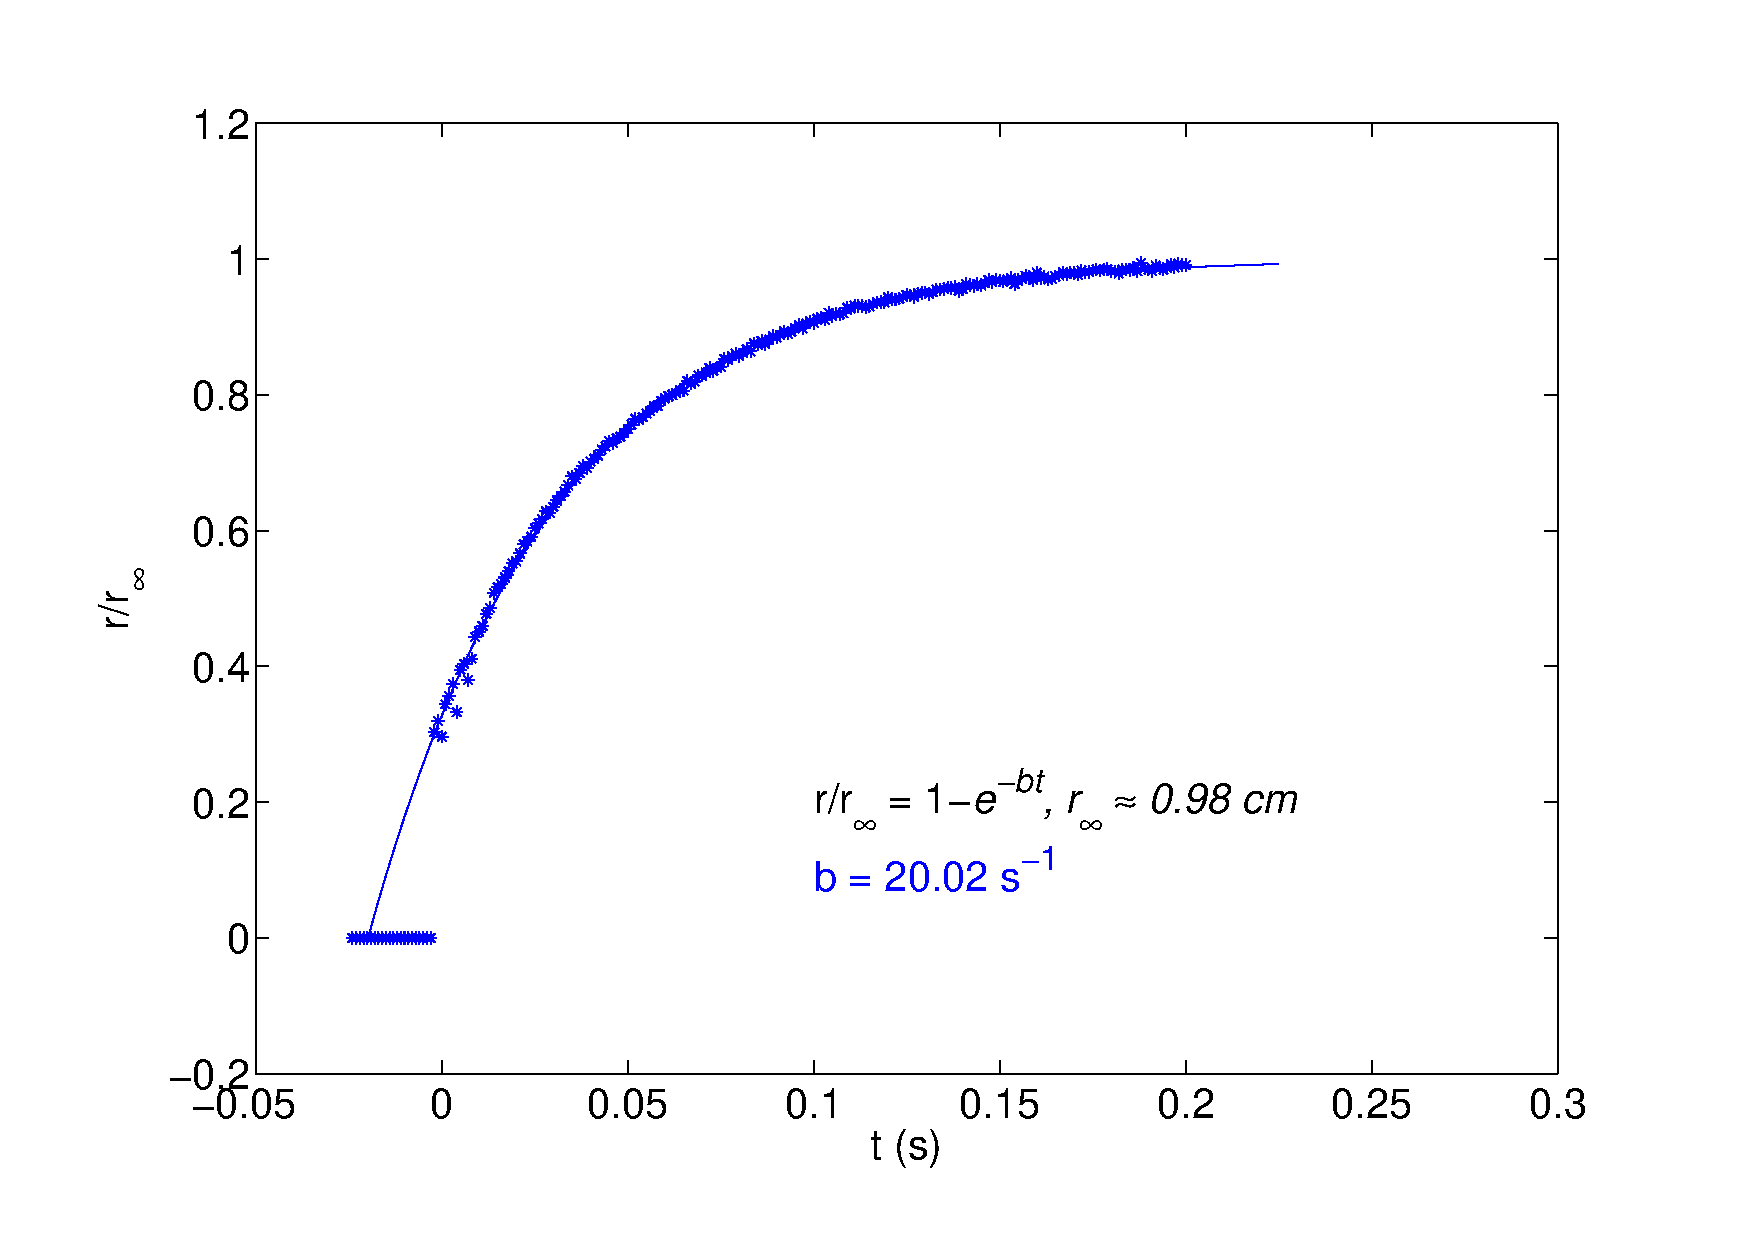
\includegraphics[scale=0.3]{roi_1mm_250mm.pdf}
       \caption{Radius of Influence for 1 mm}
       \label{fig:roi1mm}
	\end{subfigure}
	\hfill
	\begin{subfigure}[h]{0.5\textwidth}
    \centering
       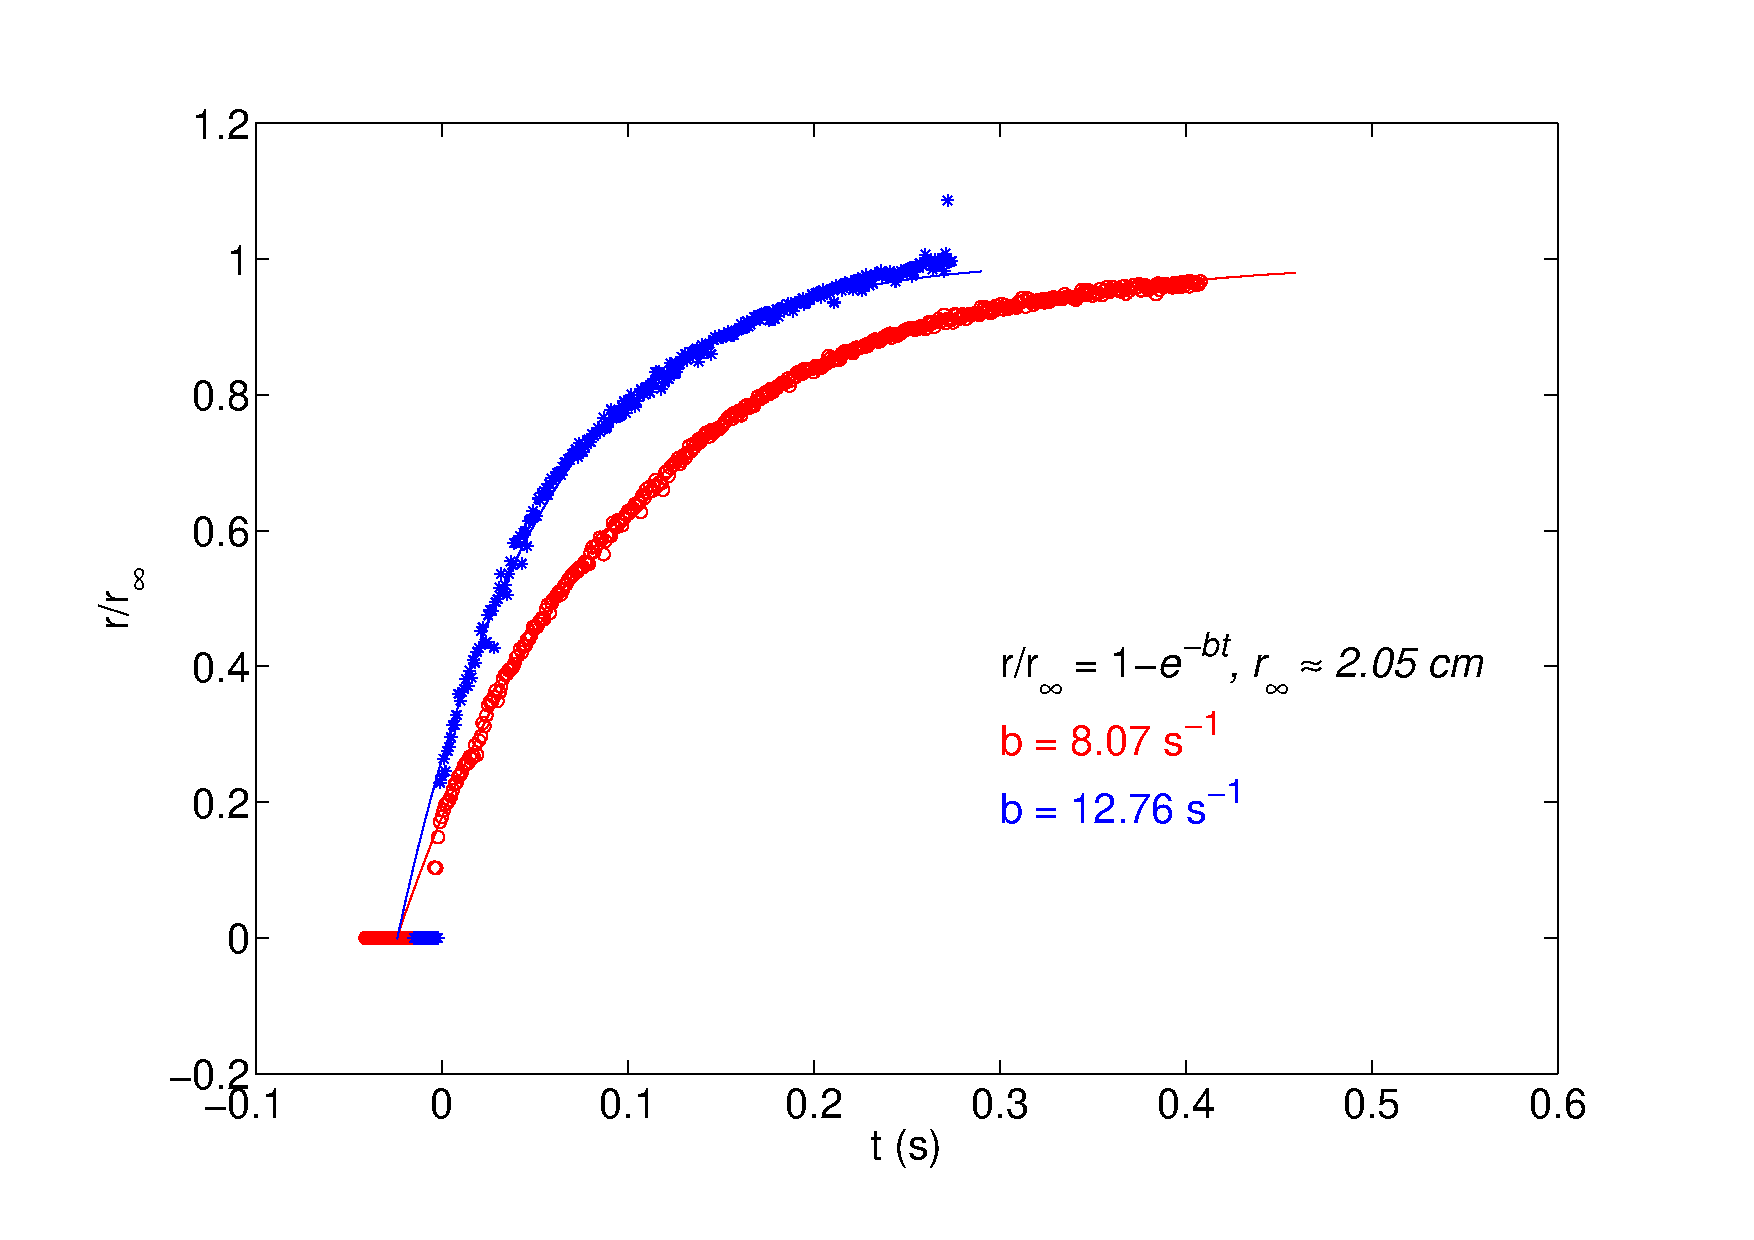
\includegraphics[scale=0.3]{roi_2mm_250mm.pdf}
       \caption{Radius of Influence for 2 mm}
       \label{fig:roi2mm}
	\end{subfigure}
	\newline
	\begin{subfigure}[h]{0.5\textwidth}
    \centering
       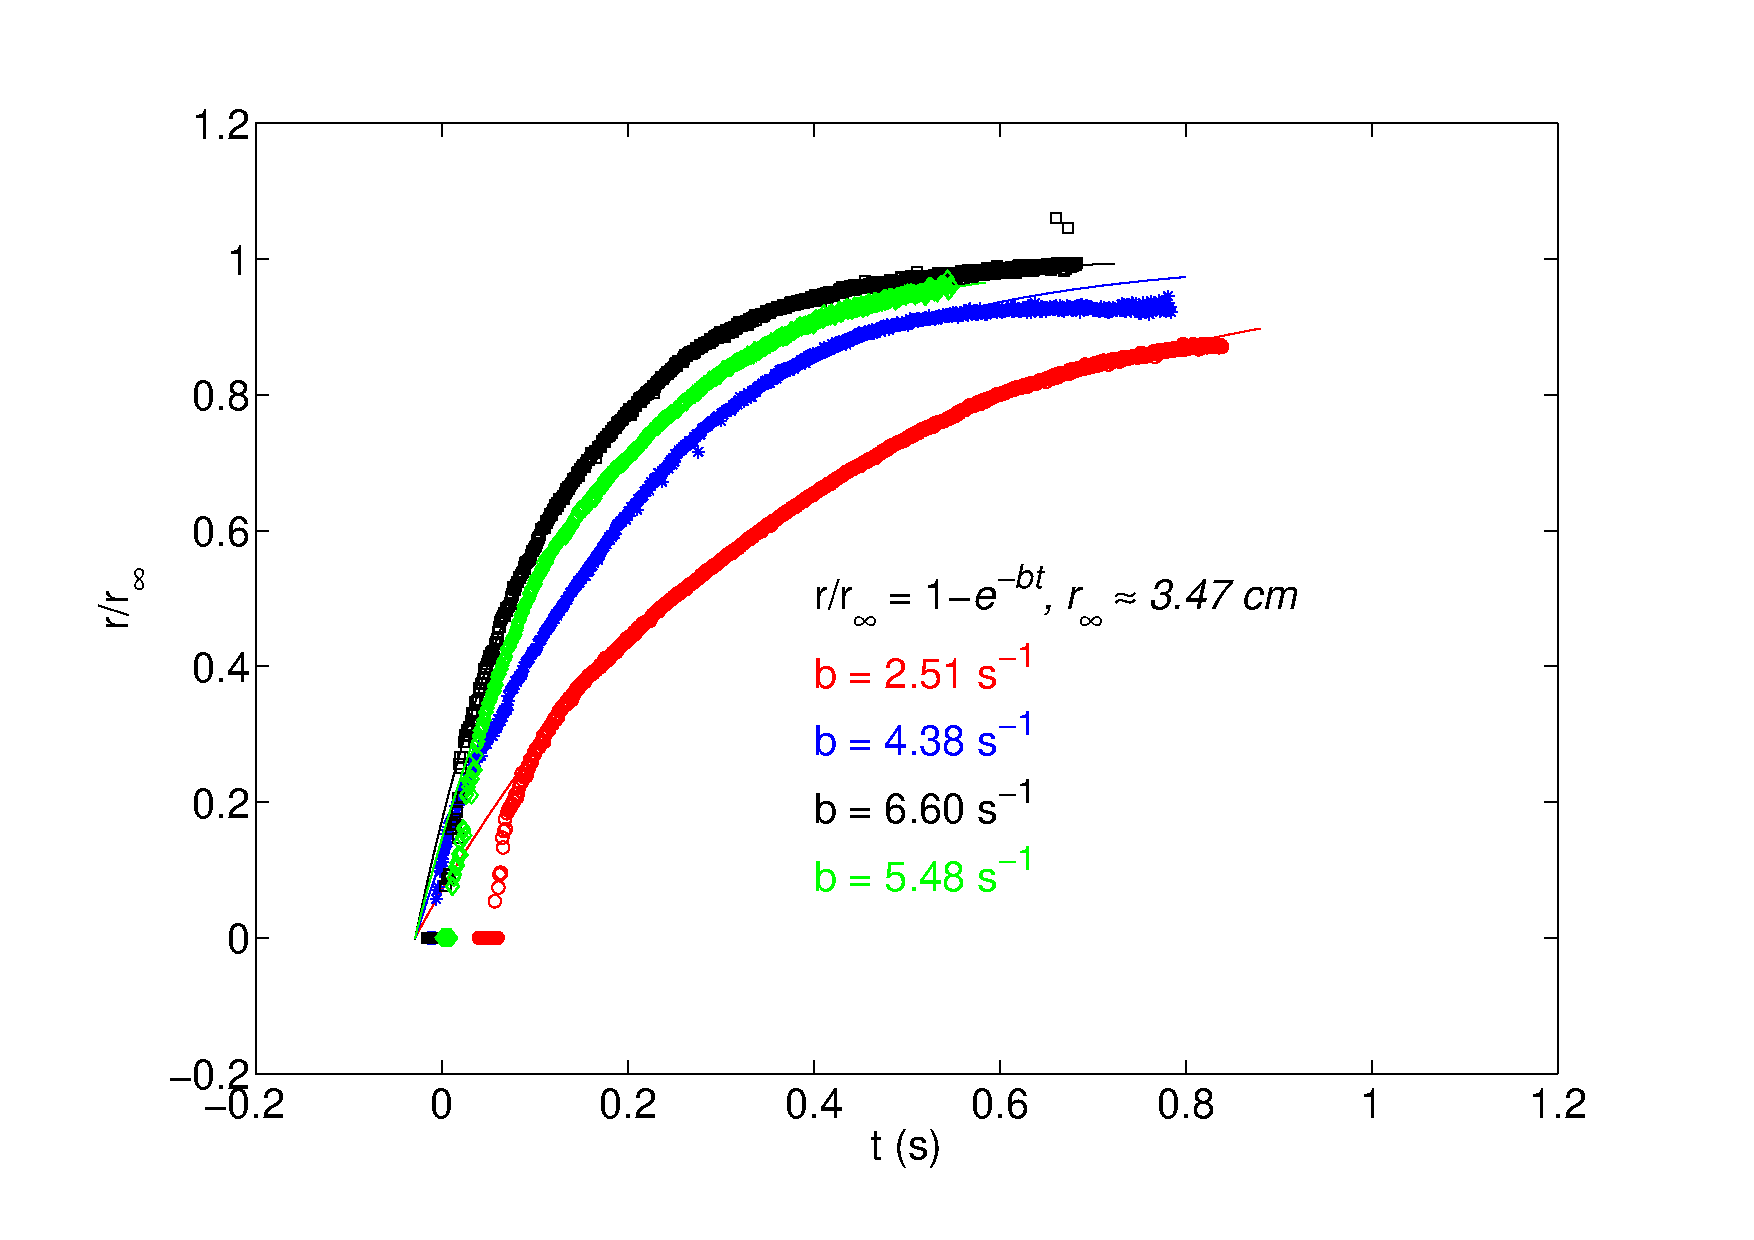
\includegraphics[scale=0.3]{roi_3mm_250mm.pdf}
       \caption{Radius of Influence for 3 mm}
       \label{fig:roi3mm}
	\end{subfigure}
	\hfill
	\begin{subfigure}[h]{0.5\textwidth}
    \centering
       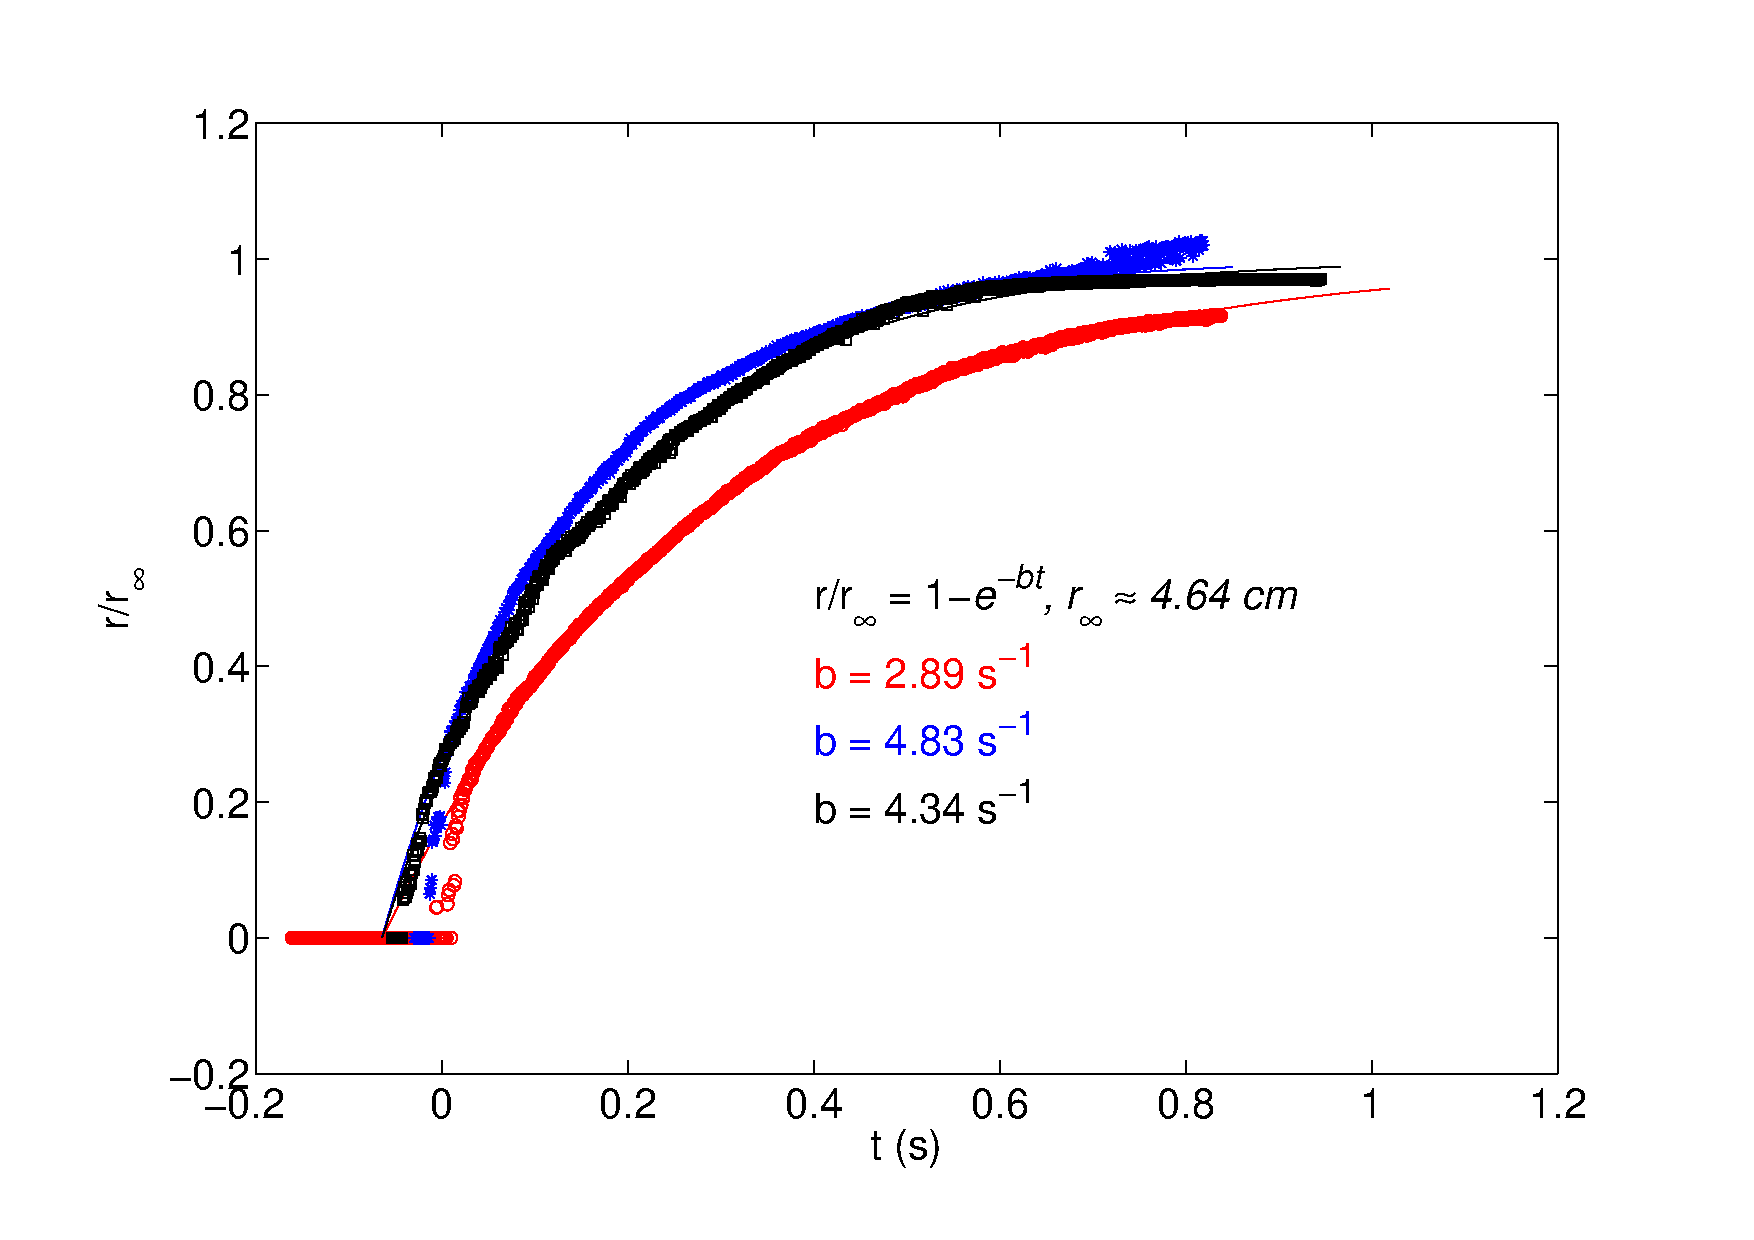
\includegraphics[scale=0.3]{roi_4mm_250mm.pdf}
       \caption{Radius of Influence for 4 mm}
       \label{fig:roi4mm}
	\end{subfigure}
	\caption{Radii of Influence for different diameters of c-boat}
	\label{fig:roiAll}
\end{figure}

\subsection{Back-of-the-Envelope Thoughts}
When a drop of surfactant is introduced on air-water interface, the surfactant molecules are drawn onto the interface to minimize the interfacial energy. The surfactant front spreads on air-water interface radially outwards with time\footnotemark[\ref{ref:mmb}] as 
\begin{equation}\label{eq:rnosub}
r(t) \approx \left(\frac{\Delta \gamma^{2}}{\mu \rho}\right)^{1/4}\ t^{3/4}
\end{equation}

Substituting $\Delta \gamma = 20 \left[\mathrm{\frac{mN}{m}}\right]$, $\mu = 10^{-3} \left[\mathrm{\frac{N.s}{m^2}}\right]$ and $\rho = 10^3 \left[\mathrm{\frac{kg}{m^3}}\right]$, we get
\begin{equation*}
r(t) \approx \alpha \ t^{3/4}
\end{equation*}
where, $\alpha = 0.14 \left[\mathrm{m.s^{-0.75}}\right]$. The rate at which area increases is, 
\begin{equation*}
\frac{\mathrm{d}}{\mathrm{dt}}A(t) = \frac{3\pi}{2}\alpha^{2}\ t^{1/2}
\end{equation*}
Effectively, one can think of sublimation as a process decreasing the surface area at a rate, $kA(t)$ where $k$ is the sublimation rate and $A(t)$ area.
Now one can write the rate equation for the effective area as,
\begin{align*}
\frac{\mathrm{d}}{\mathrm{dt}}A_{\mathrm{eff}}(t) &= \frac{\mathrm{d}}{\mathrm{dt}}A(t) - kA(t) \\
\frac{\mathrm{d}}{\mathrm{dt}}A_{\mathrm{eff}}(t) &= \pi \alpha^{2}\left(\frac{3}{2}t^{1/2}-kt^{3/2}\right)
\end{align*}
Integrating we get,
\begin{equation*}
A_{\mathrm{eff}}(t) = \pi \alpha^{2}\left(t^{3/2}-\frac{2k}{5}t^{5/2}\right)
\end{equation*}
Assuming $A_{\mathrm{eff}}(t) = \pi r_{\mathrm{eff}}^{2}$, we get 
\begin{equation}\label{eq:rsub}
r_{\mathrm{eff}}(t) = \alpha \sqrt{t^{3/2}-\frac{2k}{5}t^{5/2}}
\end{equation}
As $k\to0$, equation~\ref{eq:rsub} reduces to equation~\ref{eq:rnosub}. Note that depending on the sublimation rate $k$, the above equation yields un-physical results. The time beyond which the above equation yields un-physical results is the time taken to reach steady state saturation value for $r_{\mathrm{eff}}$ as seen in our experiments. We can obtain the value of sublimation rate $k$ experimentally as follows. By minimizing $r_{\mathrm{eff}}$, we get
\begin{equation}
k = \frac{3}{2\tau}; \; \tau = \max_{t} \ r_{\mathrm{eff}}(t)
\end{equation}
where, $\tau$ is the time at which $r_{\mathrm{eff}}(t)$ reached the steady state value.
\begin{figure}[h]
	\begin{subfigure}[h]{0.45\textwidth}
   	\centering
       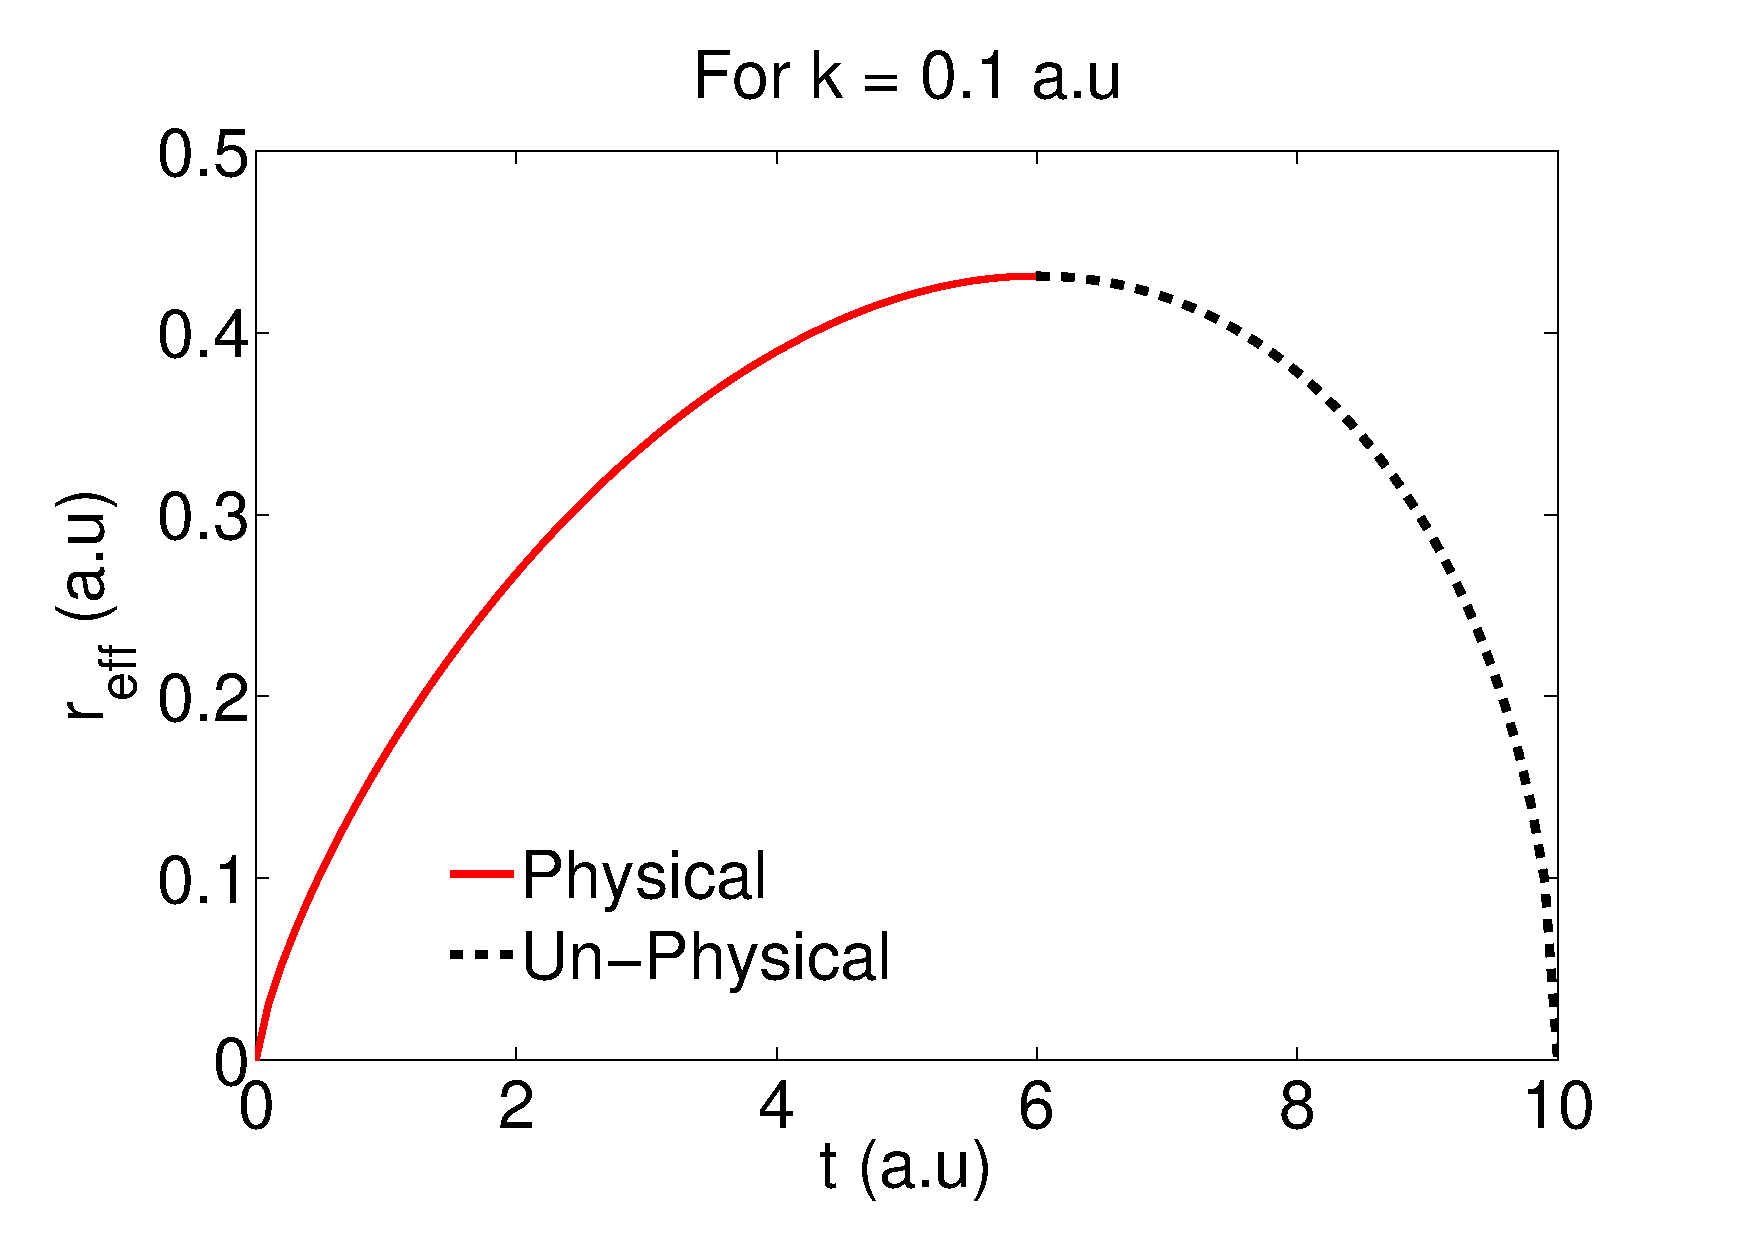
\includegraphics[scale=0.3]{kp1au.pdf}
       \caption{Proposed theoretical form of $r_{\mathrm{eff}}(t)$ given by equation~\ref{eq:rsub}}
       \label{fig:kp1au}
	\end{subfigure}
	\hfill
	\begin{subfigure}[h]{0.45\textwidth}
    \centering
       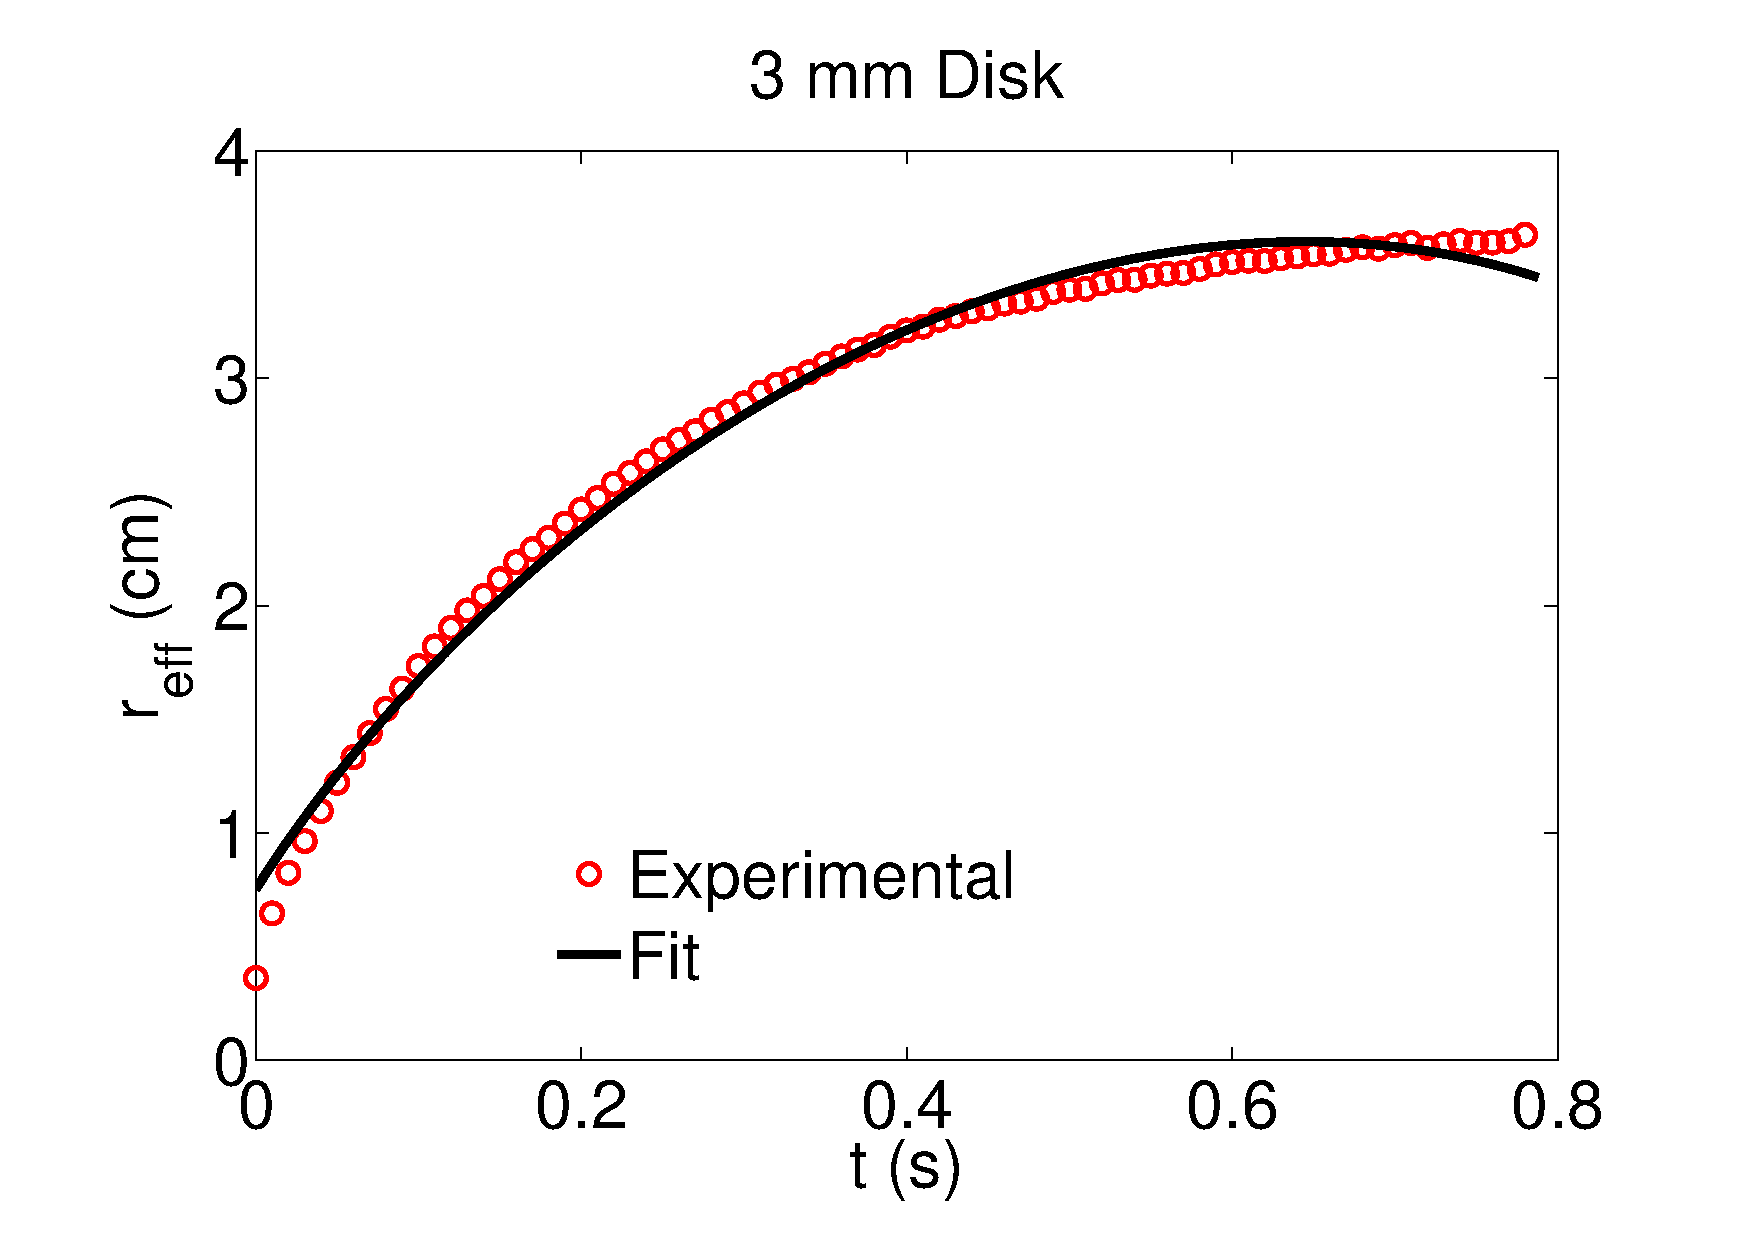
\includegraphics[scale=0.3]{theorytest_3mm.pdf}
       \caption{Experimentally measured $r_{\mathrm{eff}}(t)$ and fit to equation~\ref{eq:rsub}.}
       \label{fig:tt3mm}
	\end{subfigure}
	\caption{Hypothesized $r_{\mathrm{eff}}(t)$ and a fit to the experimental data.}
\end{figure}

\subsection{Calculation of Sublimation Rate}
Theoretically one can calculate the value of sublimation rate from the following Hertz-Langmuir-Knudsen equation.
\begin{equation}
k \approx p\sqrt{\frac{M}{2\pi R T}}
\end{equation}
where $M\left[\mathrm{kg.mol^{-1}}\right]$ is the molecular weight, $R\left[\mathrm{kg.m^{2}.s^{-2}.K^{-1}.mol^{-1}}\right]$ is the universal gas constant, $T\left[\mathrm{K}\right]$ is temperature and $p\left[\mathrm{kg.m^{-1}.s^{-2}}\right]$ is the vapor pressure. Substituting $M = 0.152 \left[\mathrm{kg.mol^{-1}}\right]$, $p = 87 \left[\mathrm{kg.m^{-1}.s^{-2}}\right]$ and $T = 298 \left[\mathrm{K}\right]$ for camphor, we get $k = 1.6 \left[\mathrm{mg.cm^{-2}.min^{-1}}\right]$.
\begin{comment}
Velocity of a boat $\approx$ 3.5 $\mathrm{cm/s}$. \\
Diameter of the boat $\approx$ 0.3 $\mathrm{cm}$. \\
The corresponding Reynold's number is, $\mathtt{Re} \approx 100$.
\end{comment}

\section{Concentration Profile in the Camphor Spread}
We know from the experiments described in the previous section that, the radial spread reaches a steady state. In this section, we attempt to derive an analytical expression for the steady state concentration profile around the camphor boat. The following derivation does not take the fluid dynamics of the underlying fluid into account rather it is accounted for through an advection term. \newline
The concentration of camphor on the surface of water can be described using the following mathematical form. 
\begin{equation}
\frac{\partial}{\partial t} c(\vec{x}, t) - \mathrm{D} \nabla^2 c(\vec{x}, t) + \vec{u}.\vec{\nabla} c(\vec{x}, t) + k c(\vec{x}, t) = 0 
\end{equation}
where, the first and second terms describe the diffusion of camphor, third term is the advection of camphor molecules due to the flow set up by the Marangoni forces and the last term is due to the evaporation of camphor into the room. \newline 
For steady state $\frac{\partial c}{\partial t} = 0$ and in 1-D the equation simplifies to
\begin{equation}
\mathrm{D} \frac{d^2}{d x^2} c(x) - u \frac{d}{dx}c(x) - k c(x) = 0
\end{equation}
We know from experiments that, the amount of camphor transported via advection is lot more than via diffusion, i.e. $\mathrm{D} \frac{d^2}{d x^2} c(x) \ll u \frac{d}{dx}c(x)$. Therefore,
\begin{equation*}
\frac{d}{dx}c(x) = -\frac{k}{u}c(x)
\end{equation*}
Solving the above equation yields, 
\begin{equation}
c(x) = \exp\left(-\frac{k}{u}x\right) + \mathrm{const.}
\end{equation}
\section{Lifetime of the c-boats}
The forces acting on a c-boat are, 1. Marangoni forces due to the surface tension gradients, which are in turn caused by the concentration gradients 2. Drag force due to the viscosity of medium. As a function of time, camphor sublimes from the c-boats and the velocity of the c-boat decreases with time. Figure~\ref{fig:cblife} shows the plot of the velocity of the c-boat as a function of time for three different trials. As camphor sublimes, the physical characteristics of the system change continuously. The life time of the c-boat sets an upper bound on the duration of an experiment. Therefore, data collection must be done within \emph{few} minutes from the beginning of the experiment.   

\begin{figure}[h]
    \begin{center}
       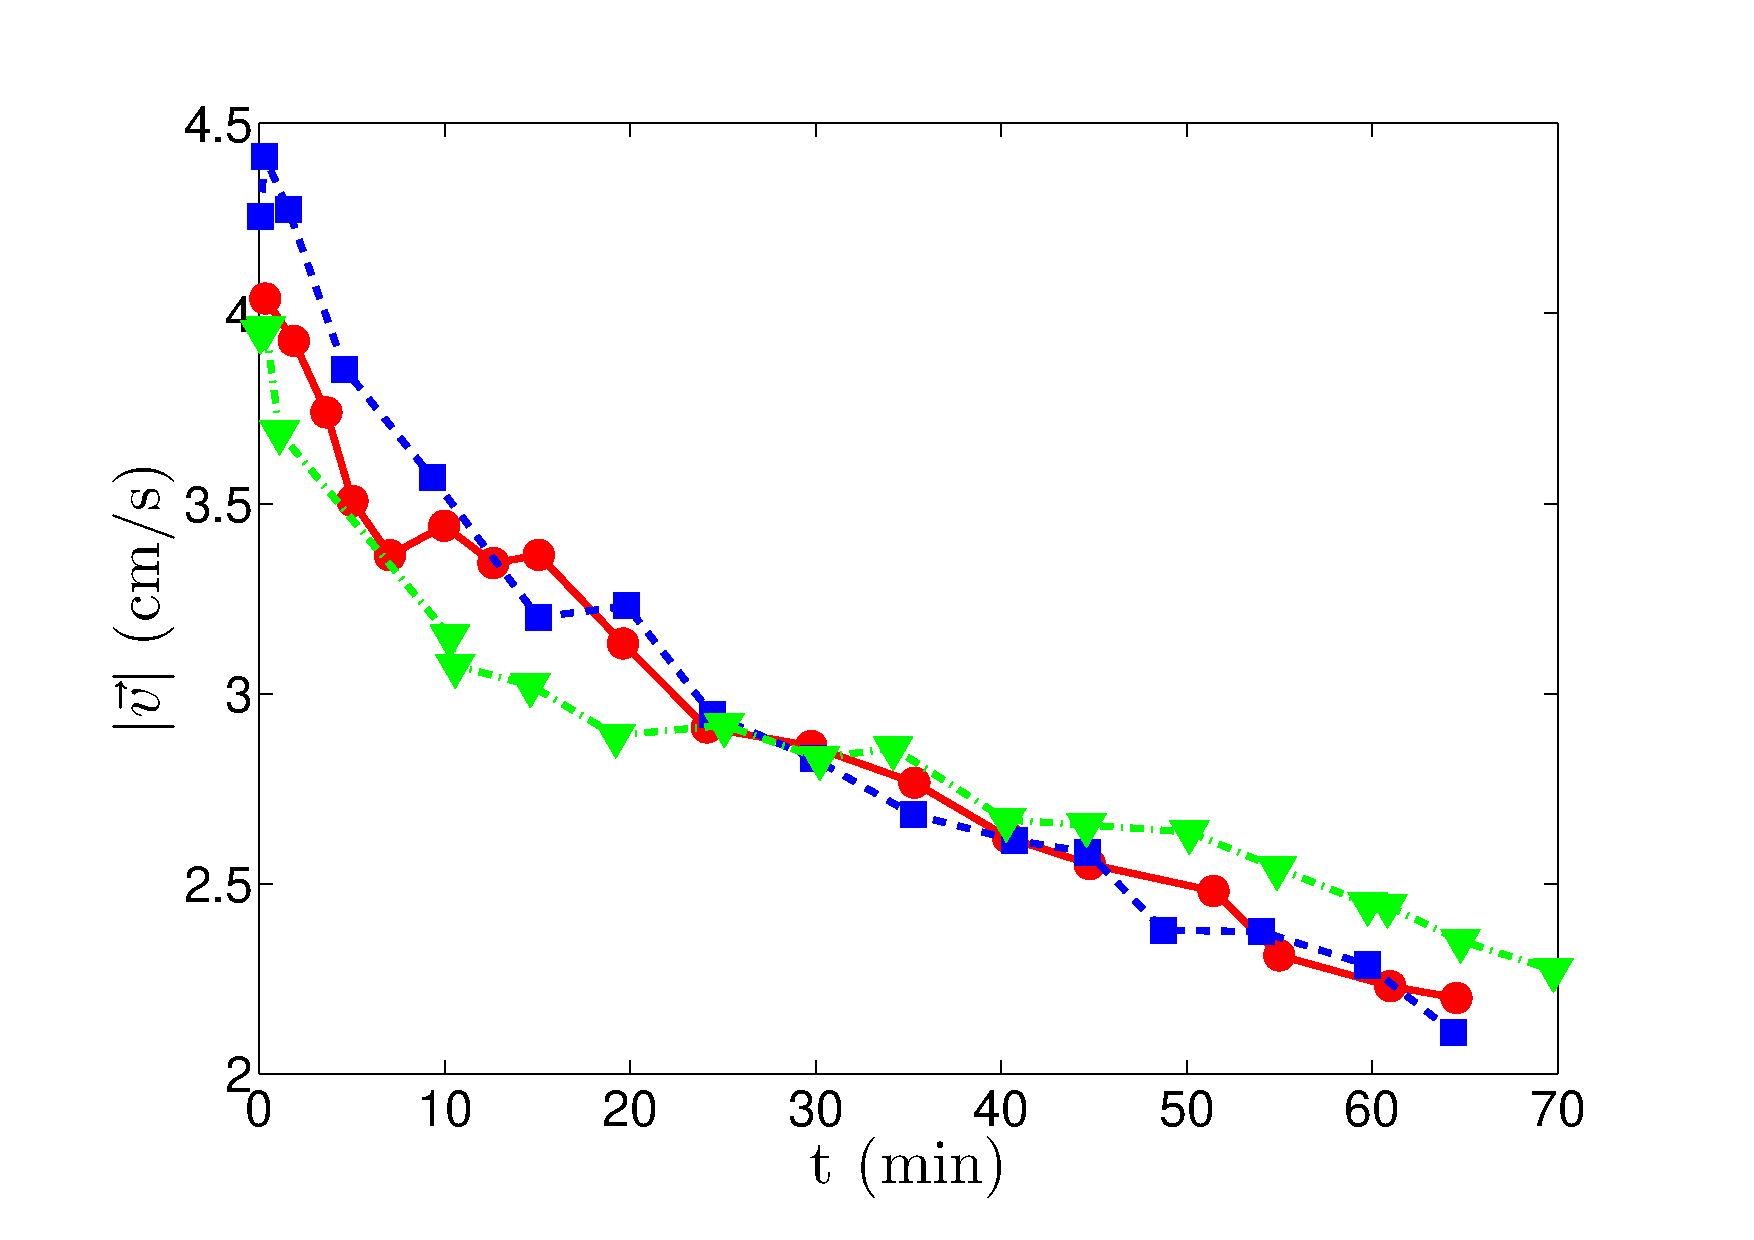
\includegraphics[scale=0.5]{cb_lifetime.pdf}
    \end{center}
    \caption{$|\vec{v}|$ of camphor boat as a function of time. The physical characteristics of the system change continuously with time.}
    \label{fig:cblife}
\end{figure}
\newpage
\section{Dynamics of the c-boats}
\subsection{Quantifying the Dynamics}
One of the goals of the project is to understand and study the collective behavior of the c-boats system. In order to quantify the collective behavior, we chose the average of speed distributions of the c-boats. One can also choose other physical quantities describing the collective behavior, such as, 1. average kinetic energy per c-boat (which is similar to a thermodynamic system where temperature is the average kinetic energy), 2. auto- or cross-correlations of positions or velocities, 3. Fourier spectrum of the positions (for a crystal in any dimension, Fourier spectrum gives the periodicity in the lattice), etc. Mathematically the average of speed distributions of all the c-boats is given by,
\begin{equation}
\mathrm{Pr}\left[|\vec{v}|_{\mathrm{min}} \leq |\vec{v}| \leq |\vec{v}|_{\mathrm{max}}\right] = \sum_{i}\mathrm{Pr}_{i}\left[|\vec{v_{i}}|_{\mathrm{min}} \leq |\vec{v_{i}}| \leq |\vec{v_{i}}|_{\mathrm{max}}\right]
\end{equation}
where, $\mathrm{Pr}_{i}\left[|\vec{v_{i}}|_{\mathrm{min}} \leq |\vec{v_{i}}| \leq |\vec{v_{i}}|_{\mathrm{max}}\right]$ is the speed probability distribution function and is obtained using the histogram of $|\vec{v_{i}}|$ for the $i^\textrm{th}$ c-boat. In calculating the histogram of $|\vec{v_{i}}|$, the bin width is taken to be the smallest measurable change in speed experimentally. Figure~\ref{fig:vpdfall} shows the average of speed distributions of the c-boats as a function of number of c-boats in the system. The spread in the distribution, for small $N$, towards the smaller speed values is a boundary effect. When a c-boat approaches the boundary, it slows down or completely stops for a short amount of time ($\approx 2-5 \textrm{ s}$). Data in figure~\ref{fig:vpdfall} was collected with a 3 mm diameter c-boat in a 60 mm diameter petri dish. We are performing the same experiment in a larger petri dish (250 mm diameter). Some of the results are listed in figure~\ref{fig:vpdfall25cm}. To completely avoid the boundary effect, we calculate the speed/velocity of the c-boat at least 10-diameters away from the boundary. The choice of 10-diameters from the boundary is a result of experiments on the radial extent of camphor spread discussed in earlier sections. Note that, for different diameters of c-boats, the spread is approximately 10-times the diameter of the c-boat. The major difficulty in performing the experiment in a larger dish is the introduction of camphor boats, which usually takes longer time, before which considerable amount of camphor had sublimed from the first batch of camphor boats. 
\begin{figure}[h!]
	\begin{subfigure}[h!]{0.5\textwidth}
    \centering
       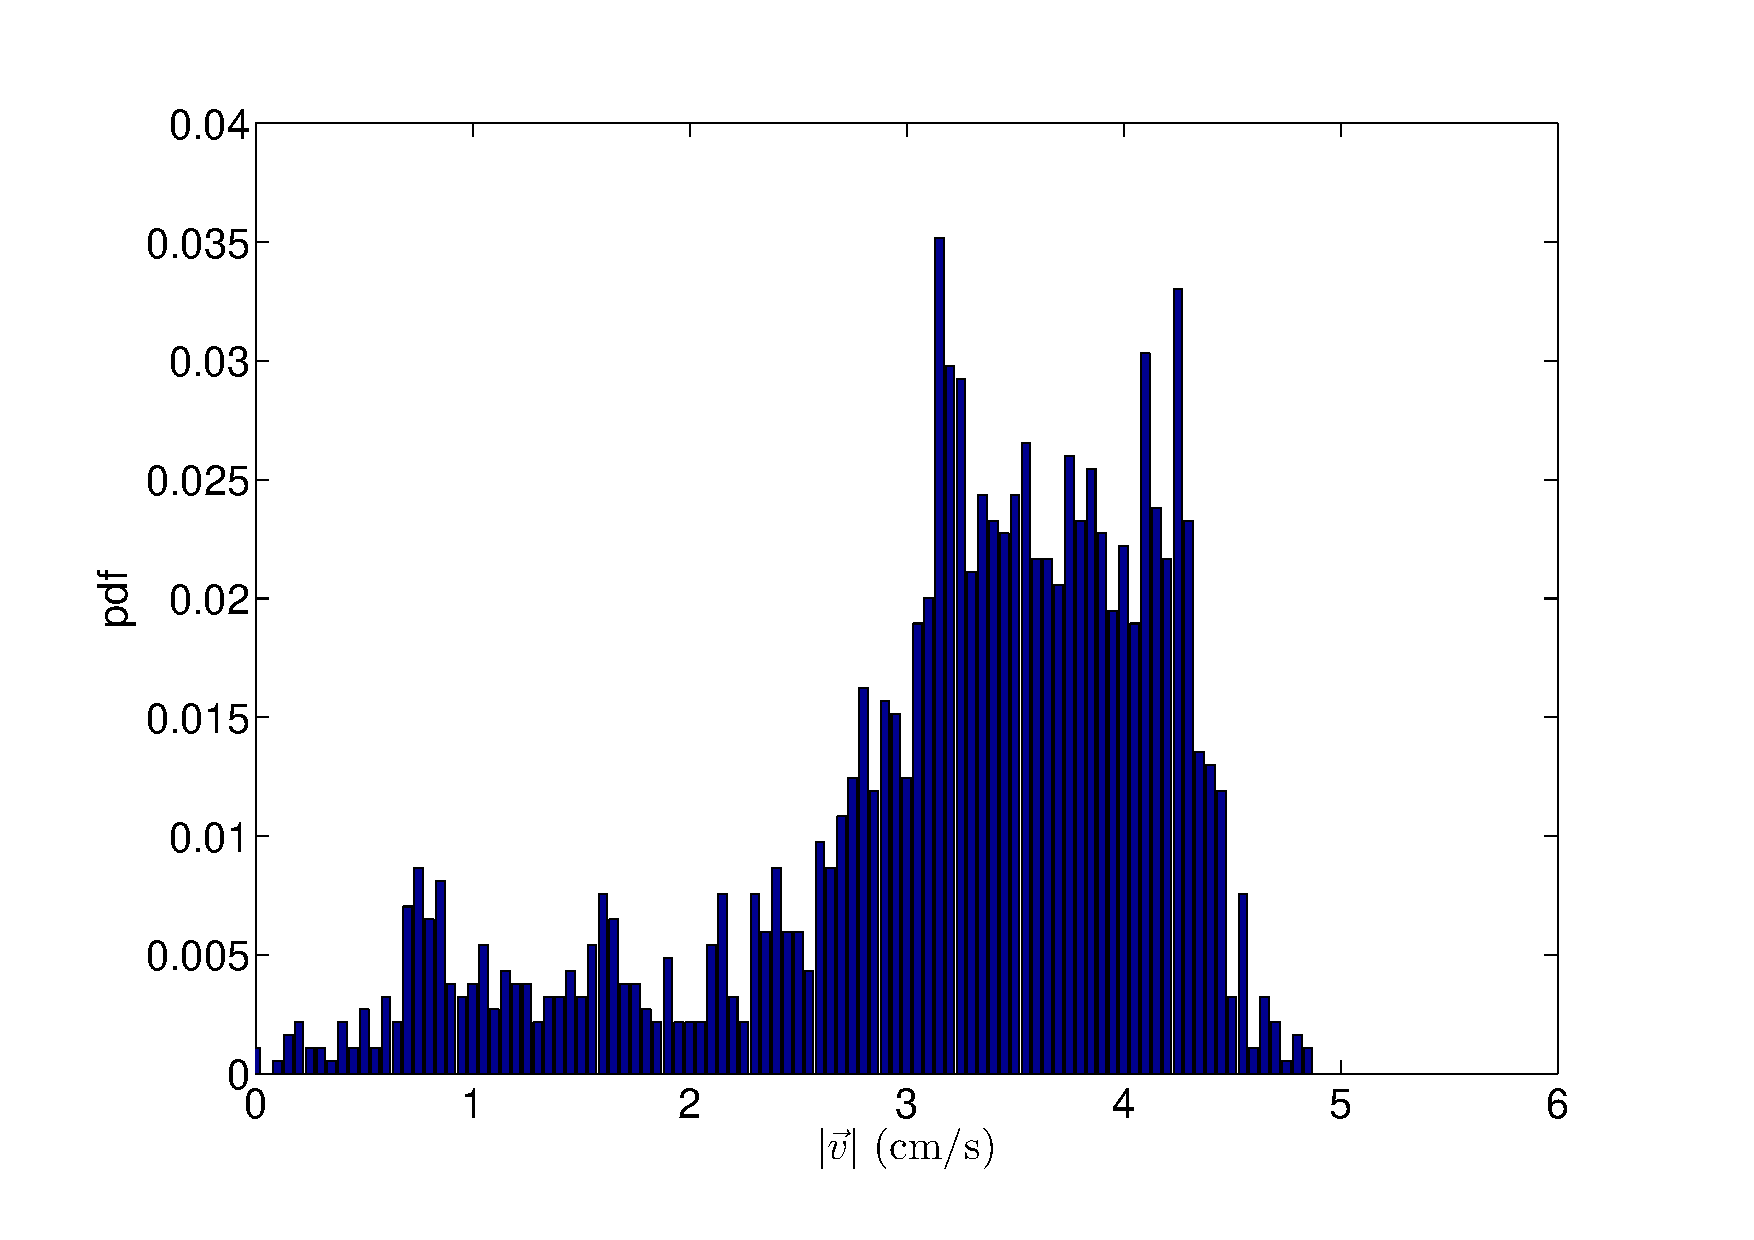
\includegraphics[scale=0.28]{cb_1_3mm_60mm_v_pdf.pdf}
       \caption{N = 1}
       \label{fig:vpdf_1}
	\end{subfigure}
	\hfill
	\begin{subfigure}[h!]{0.5\textwidth}
    \centering
       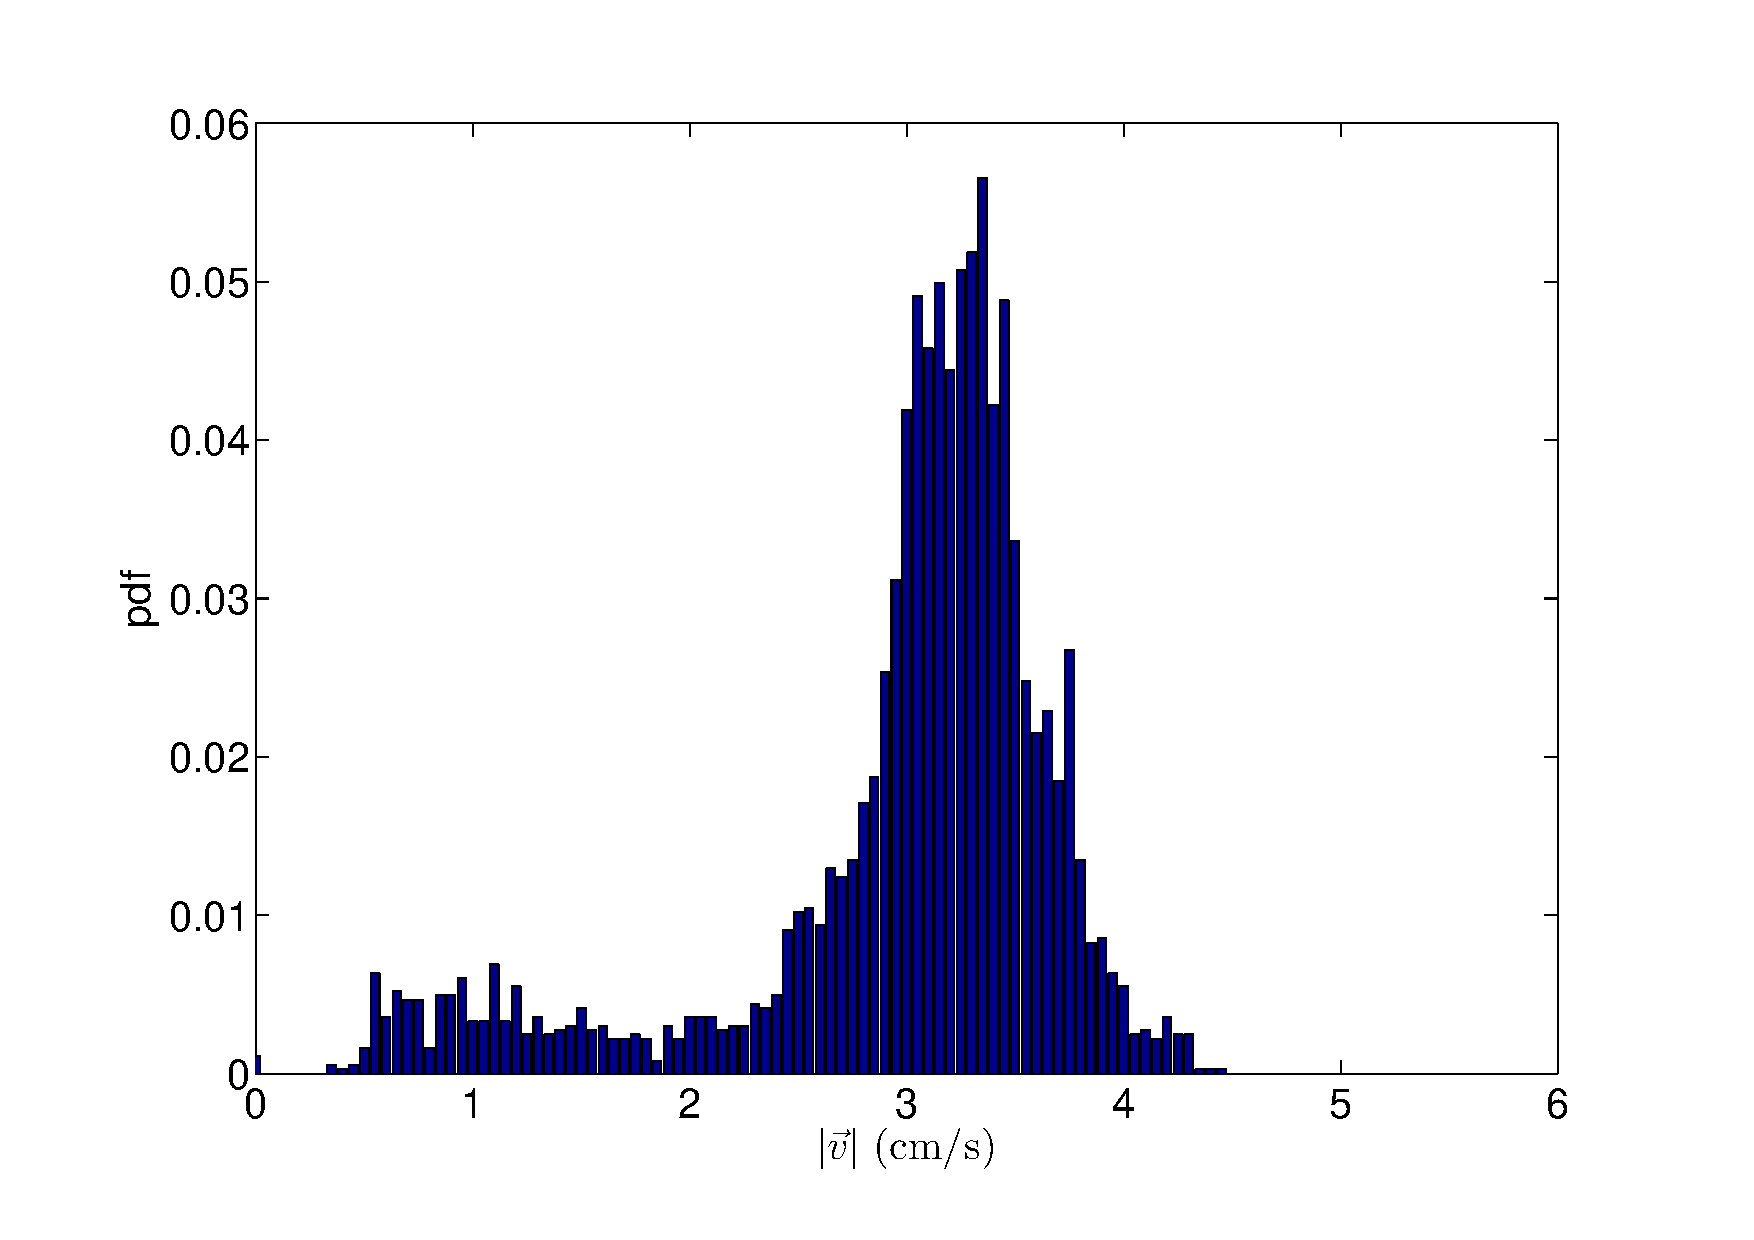
\includegraphics[scale=0.28]{cb_2_3mm_60mm_v_pdf.pdf}
       \caption{N = 2}
       \label{fig:vpdf_2}
	\end{subfigure}
	\begin{subfigure}[h!]{0.5\textwidth}
    \centering
       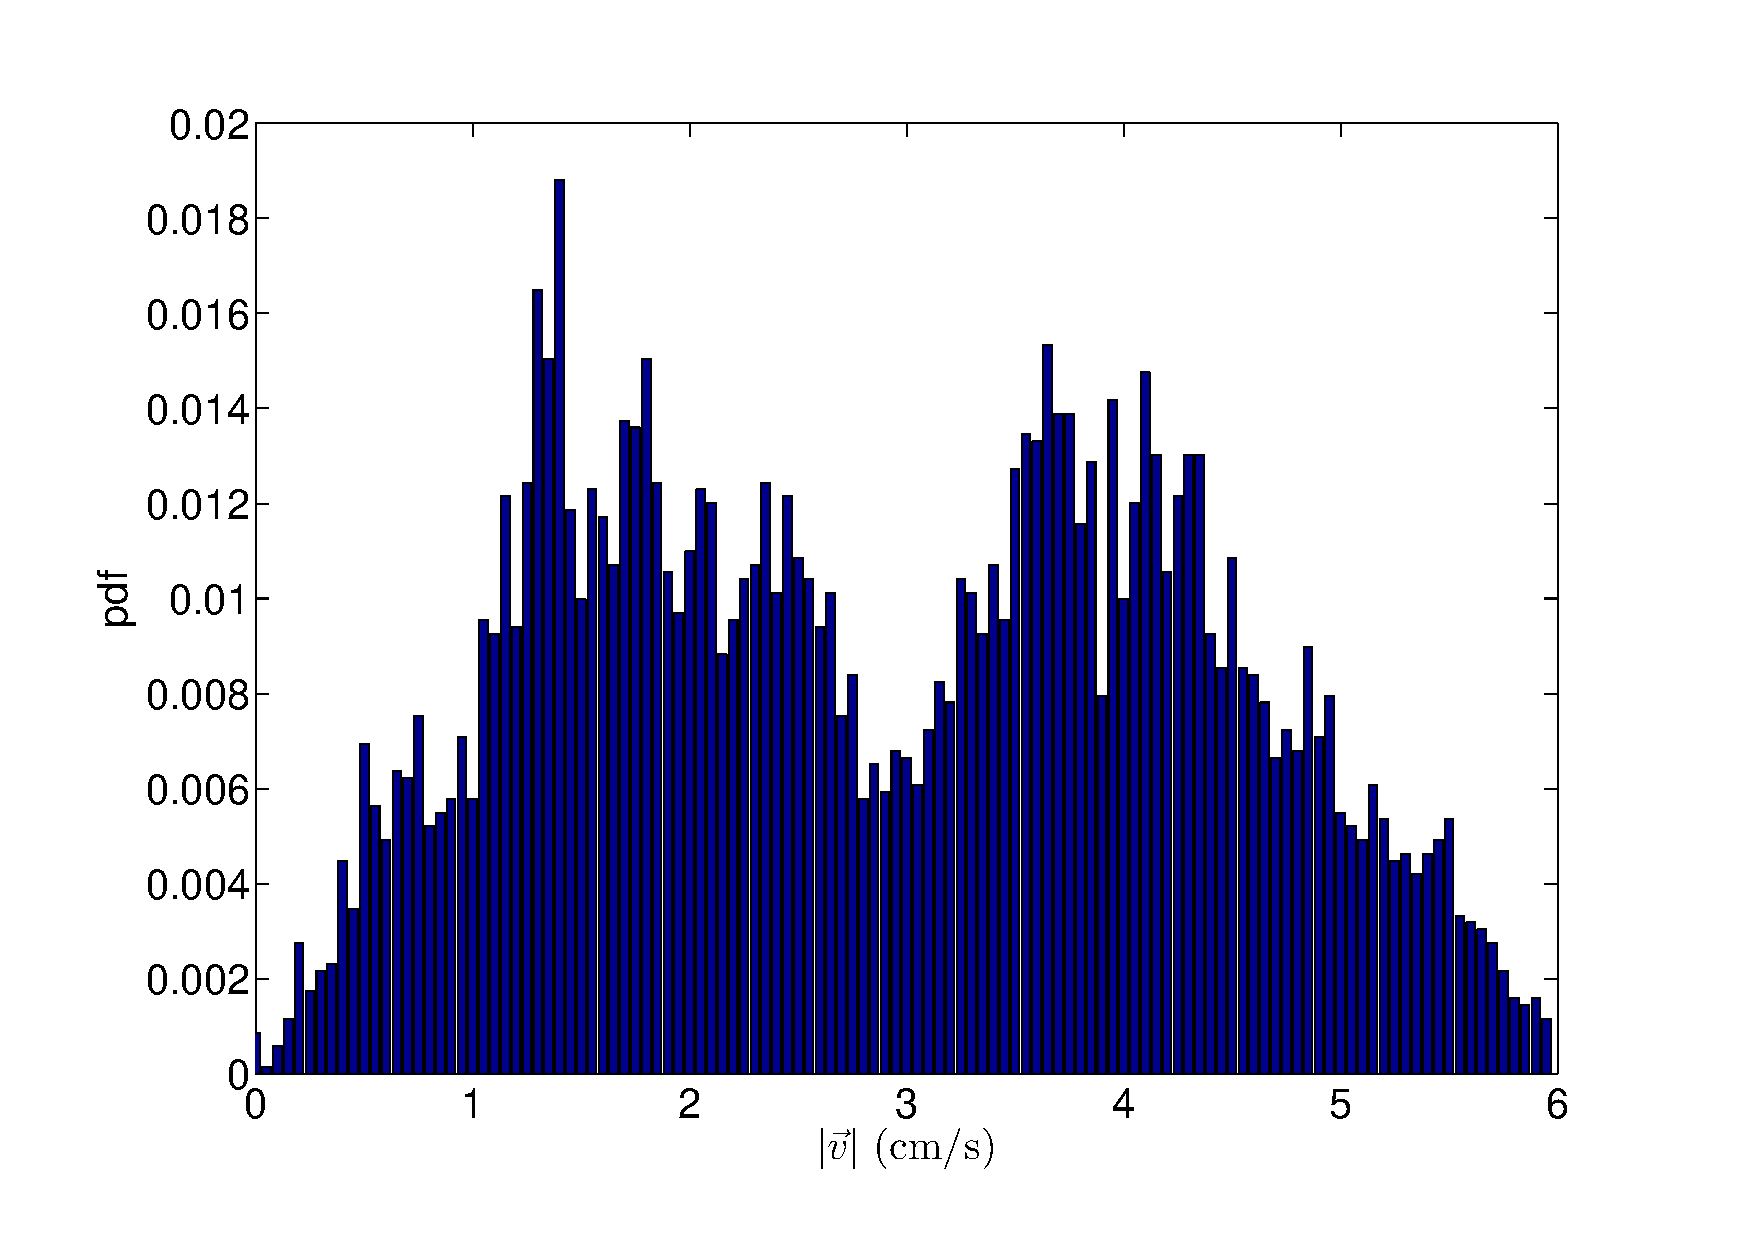
\includegraphics[scale=0.28]{cb_4_3mm_60mm_v_pdf.pdf}
       \caption{N = 4}
       \label{fig:vpdf_4}
	\end{subfigure}
	\hfill
	\begin{subfigure}[h!]{0.5\textwidth}
    \centering
       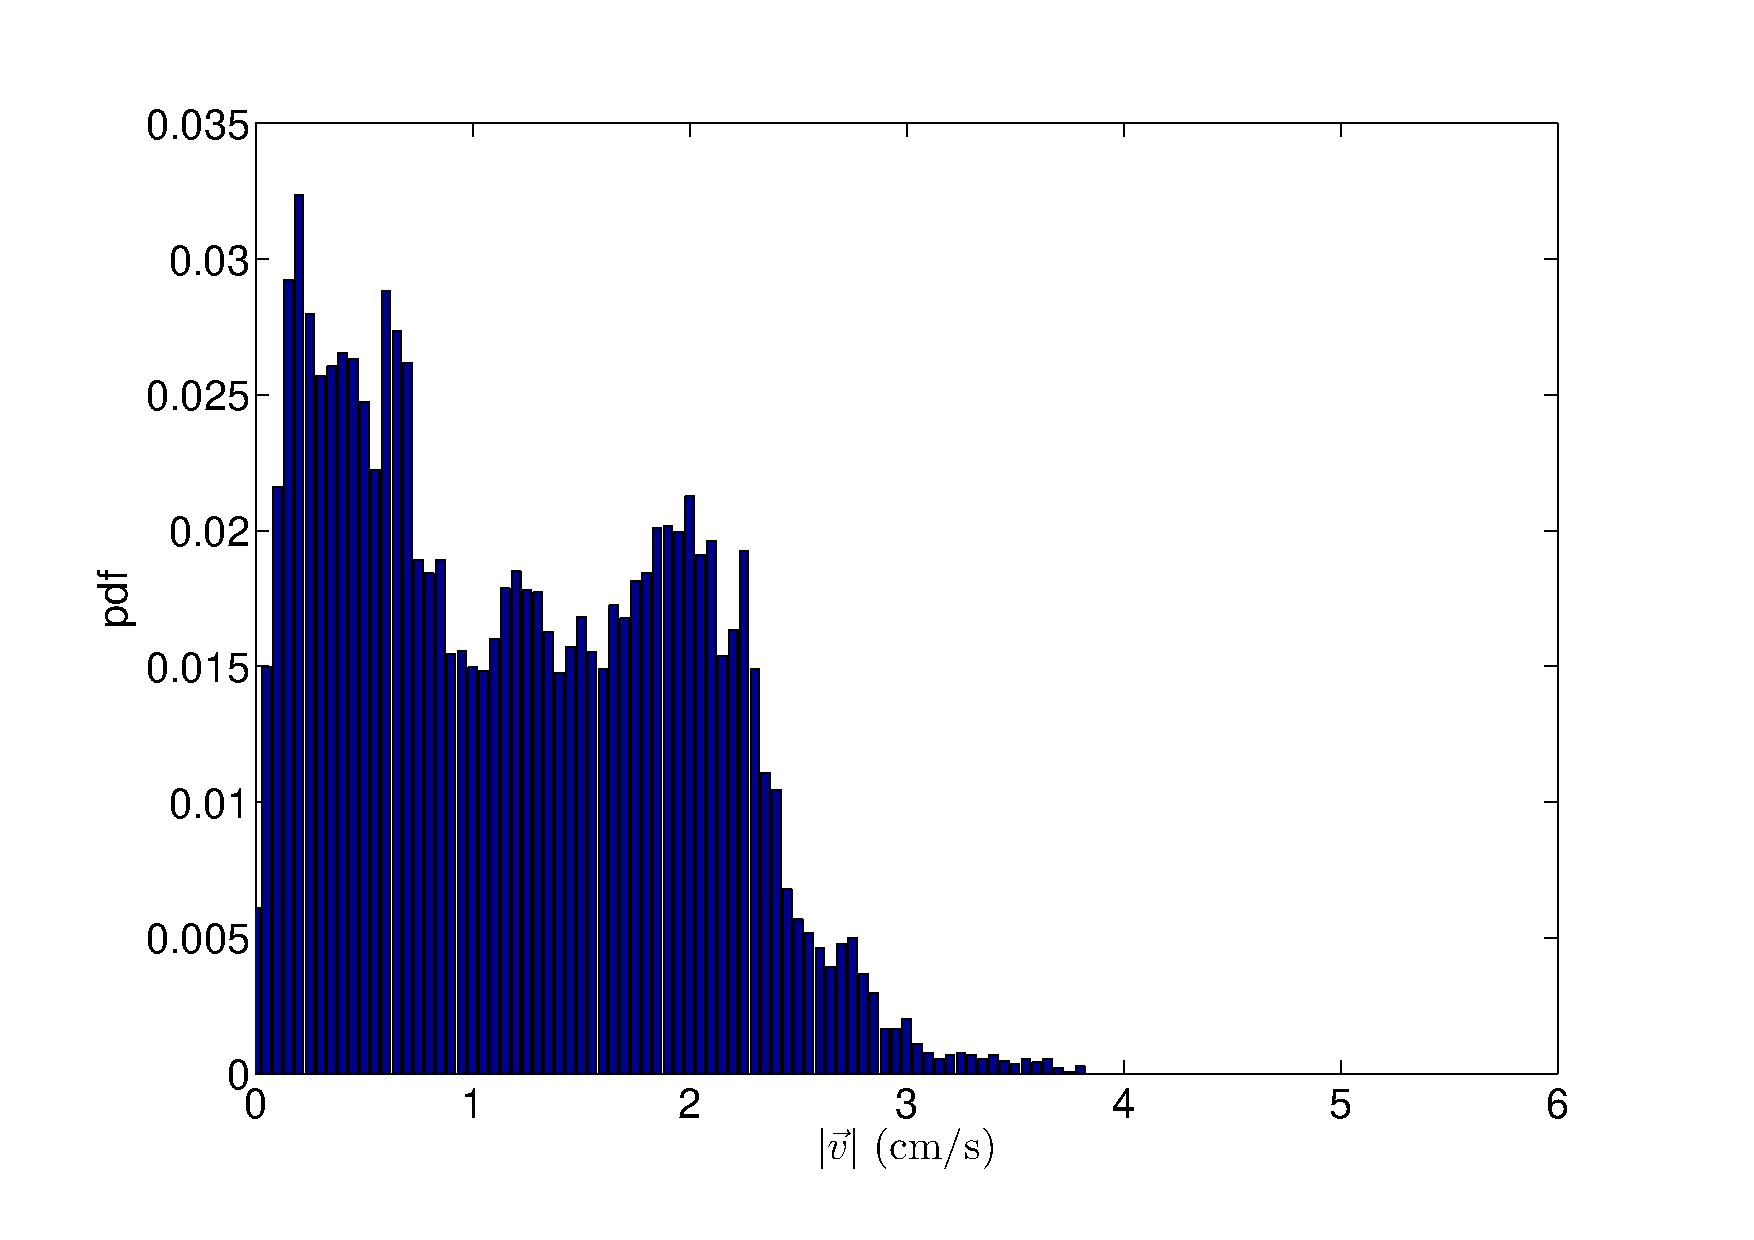
\includegraphics[scale=0.28]{cb_8_3mm_60mm_v_pdf.pdf}
       \caption{N = 8}
       \label{fig:vpdf_8}
	\end{subfigure}
	\begin{subfigure}[h!]{0.5\textwidth}
    \centering
       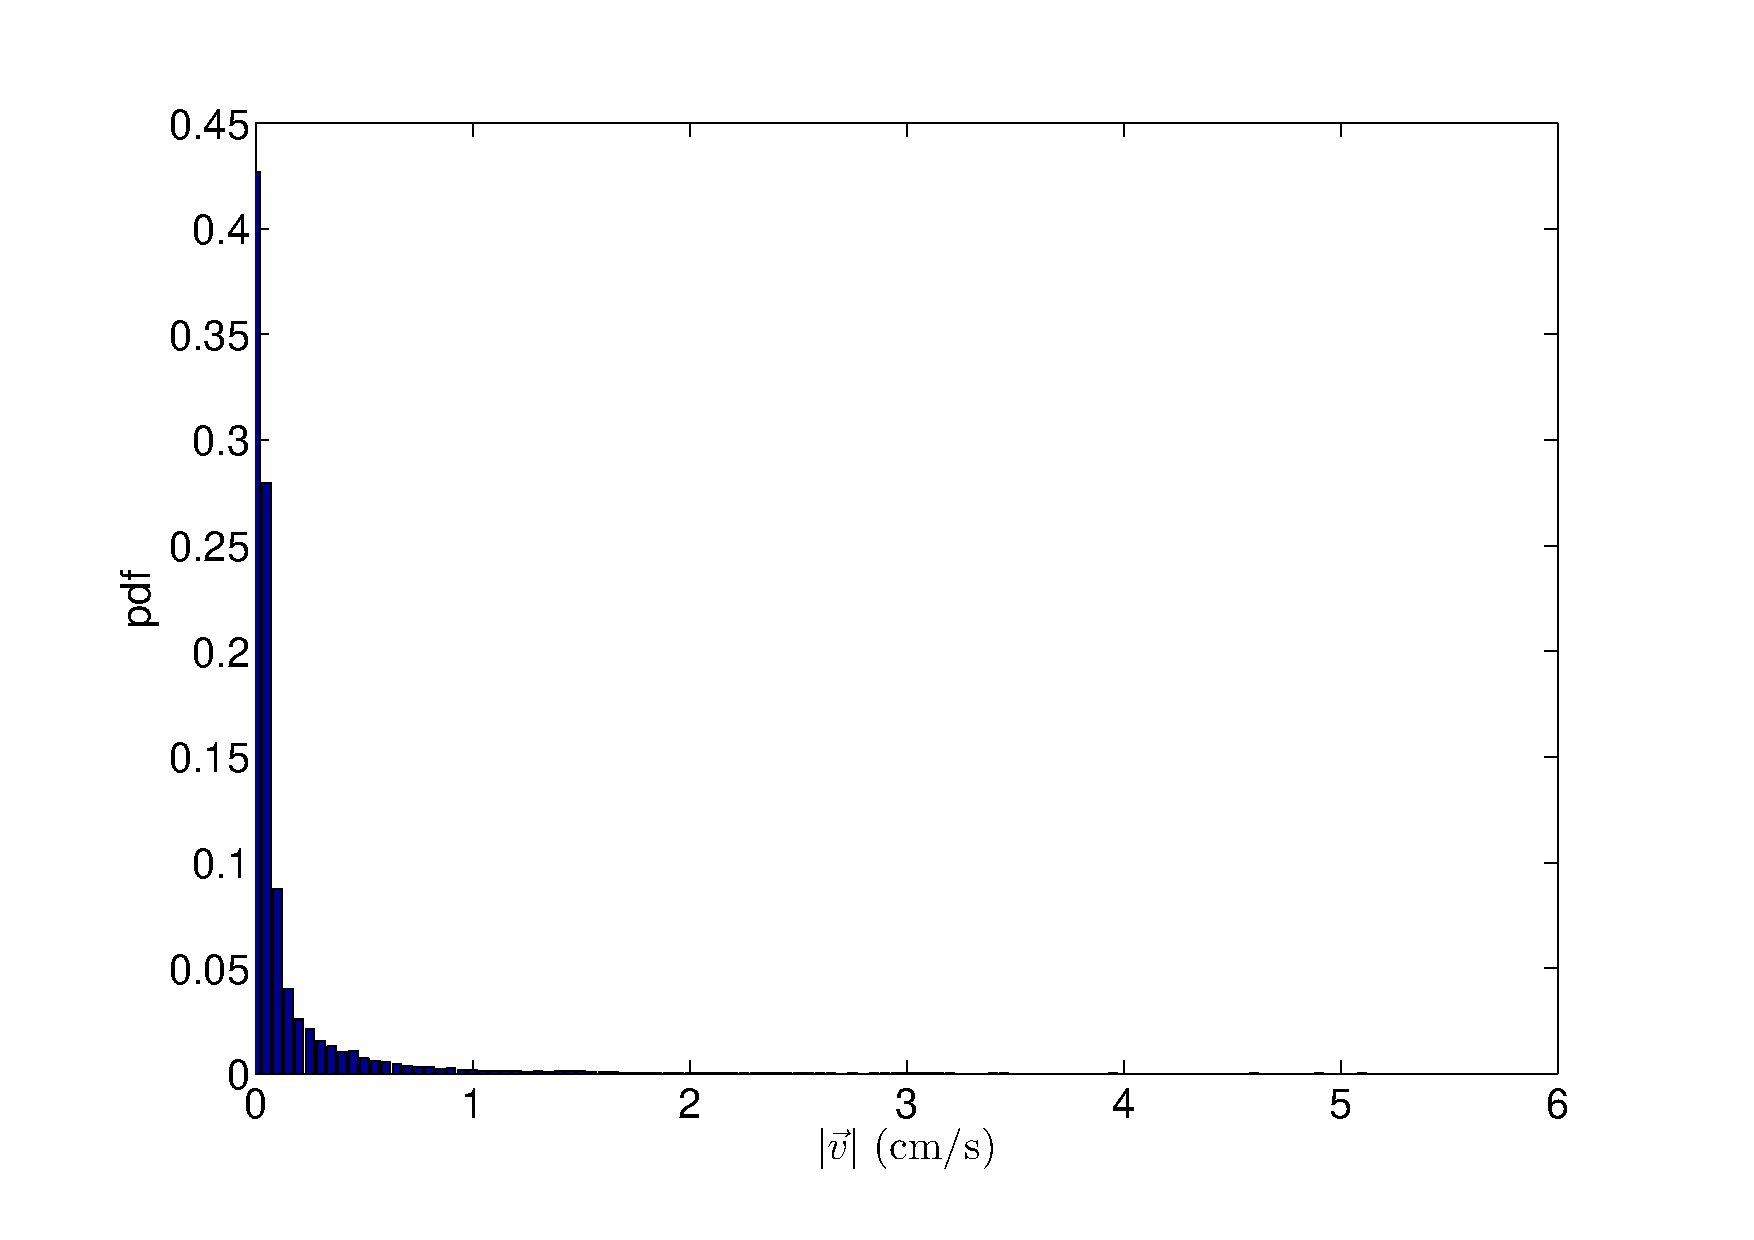
\includegraphics[scale=0.28]{cb_21_3mm_60mm_v_pdf.pdf}
       \caption{N = 21}
       \label{fig:vpdf_21}
	\end{subfigure}
	\hfill
	\begin{subfigure}[h!]{0.5\textwidth}
    \centering
       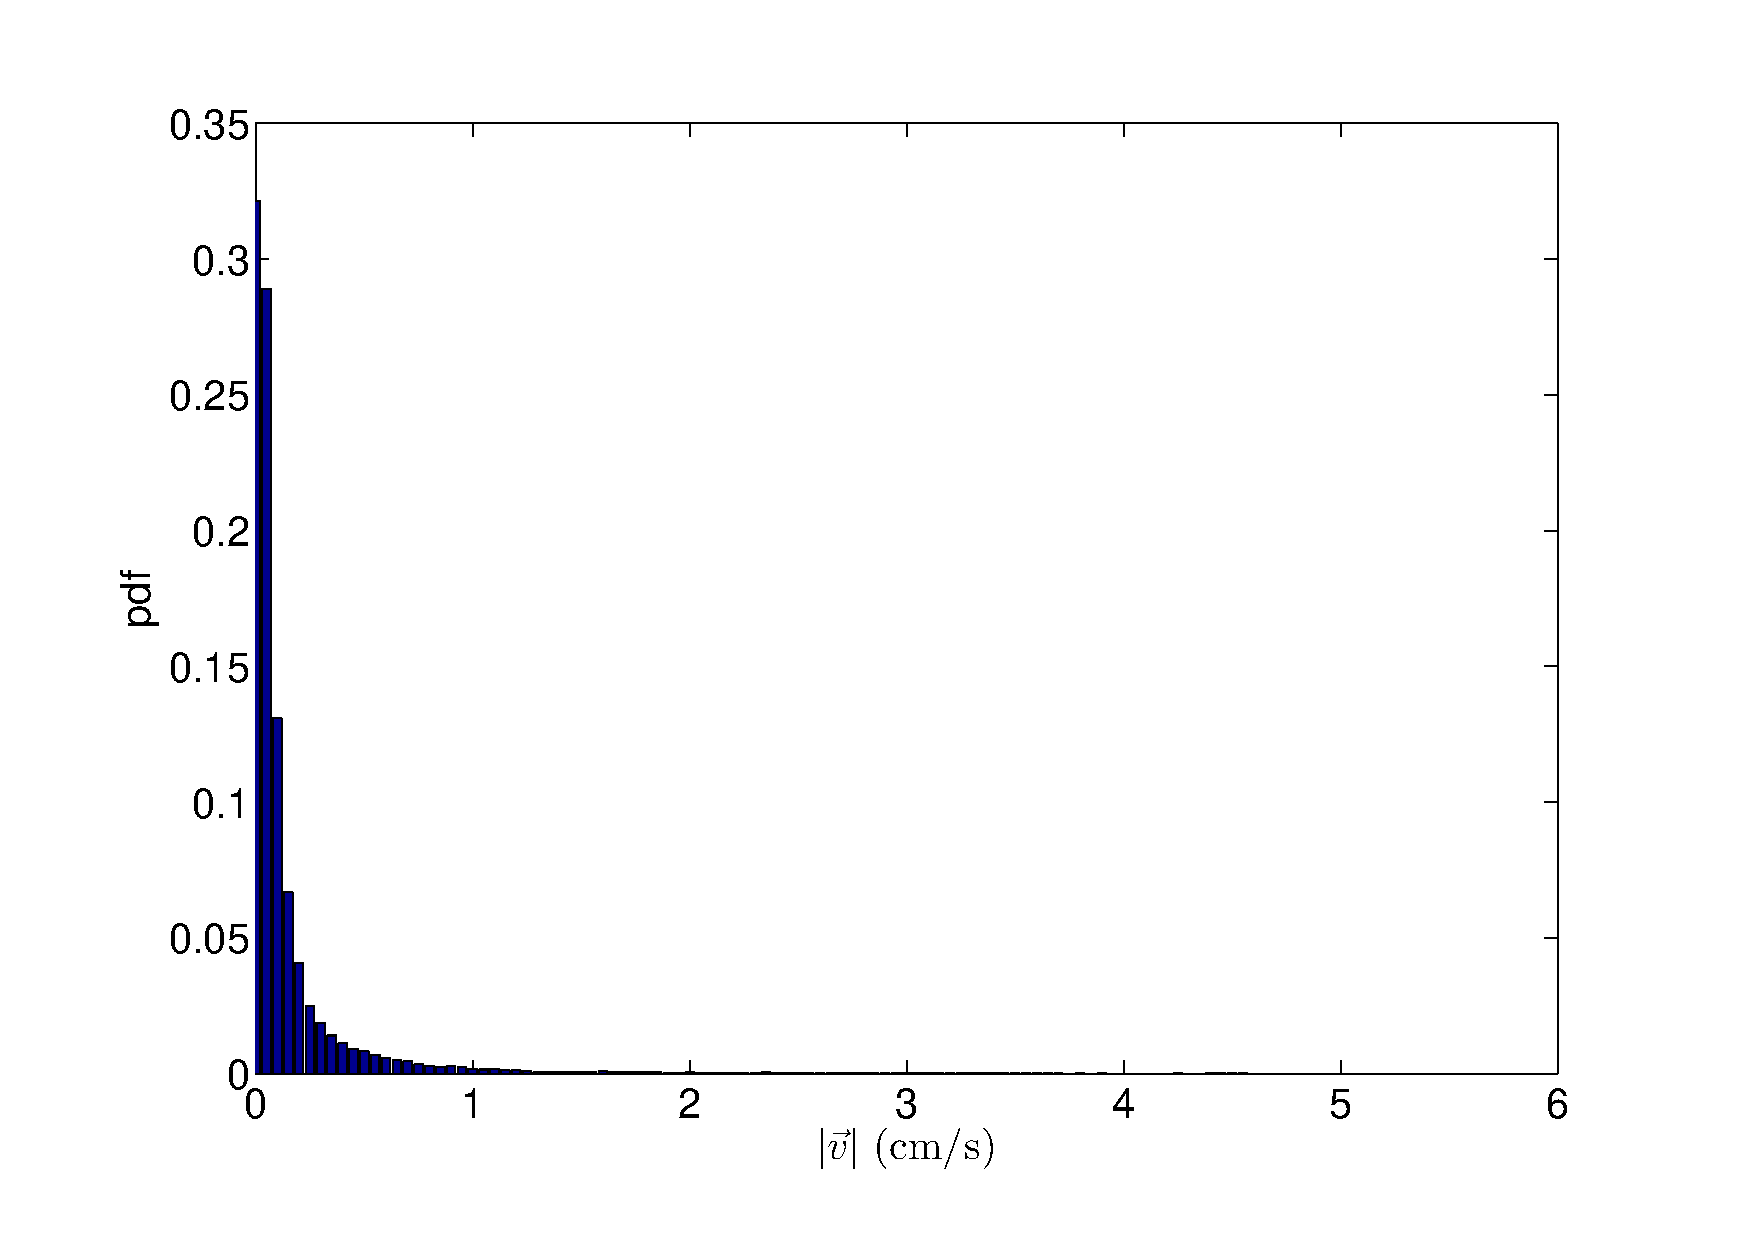
\includegraphics[scale=0.28]{cb_29_3mm_60mm_v_pdf.pdf}
       \caption{N = 29}
       \label{fig:vpdf_29}
	\end{subfigure}
	\caption{Average of speed distributions of 3 mm c-boats in a 60 mm petri dish. Note the change in the distribution as function of number of c-boats in the system. Beyond N = 21 the system is mostly in the frozen (could be glassy/crystalline) state.}
	\label{fig:vpdfall}
\end{figure}

\begin{figure}[h!]
	\begin{subfigure}[h!]{0.5\textwidth}
    \centering
       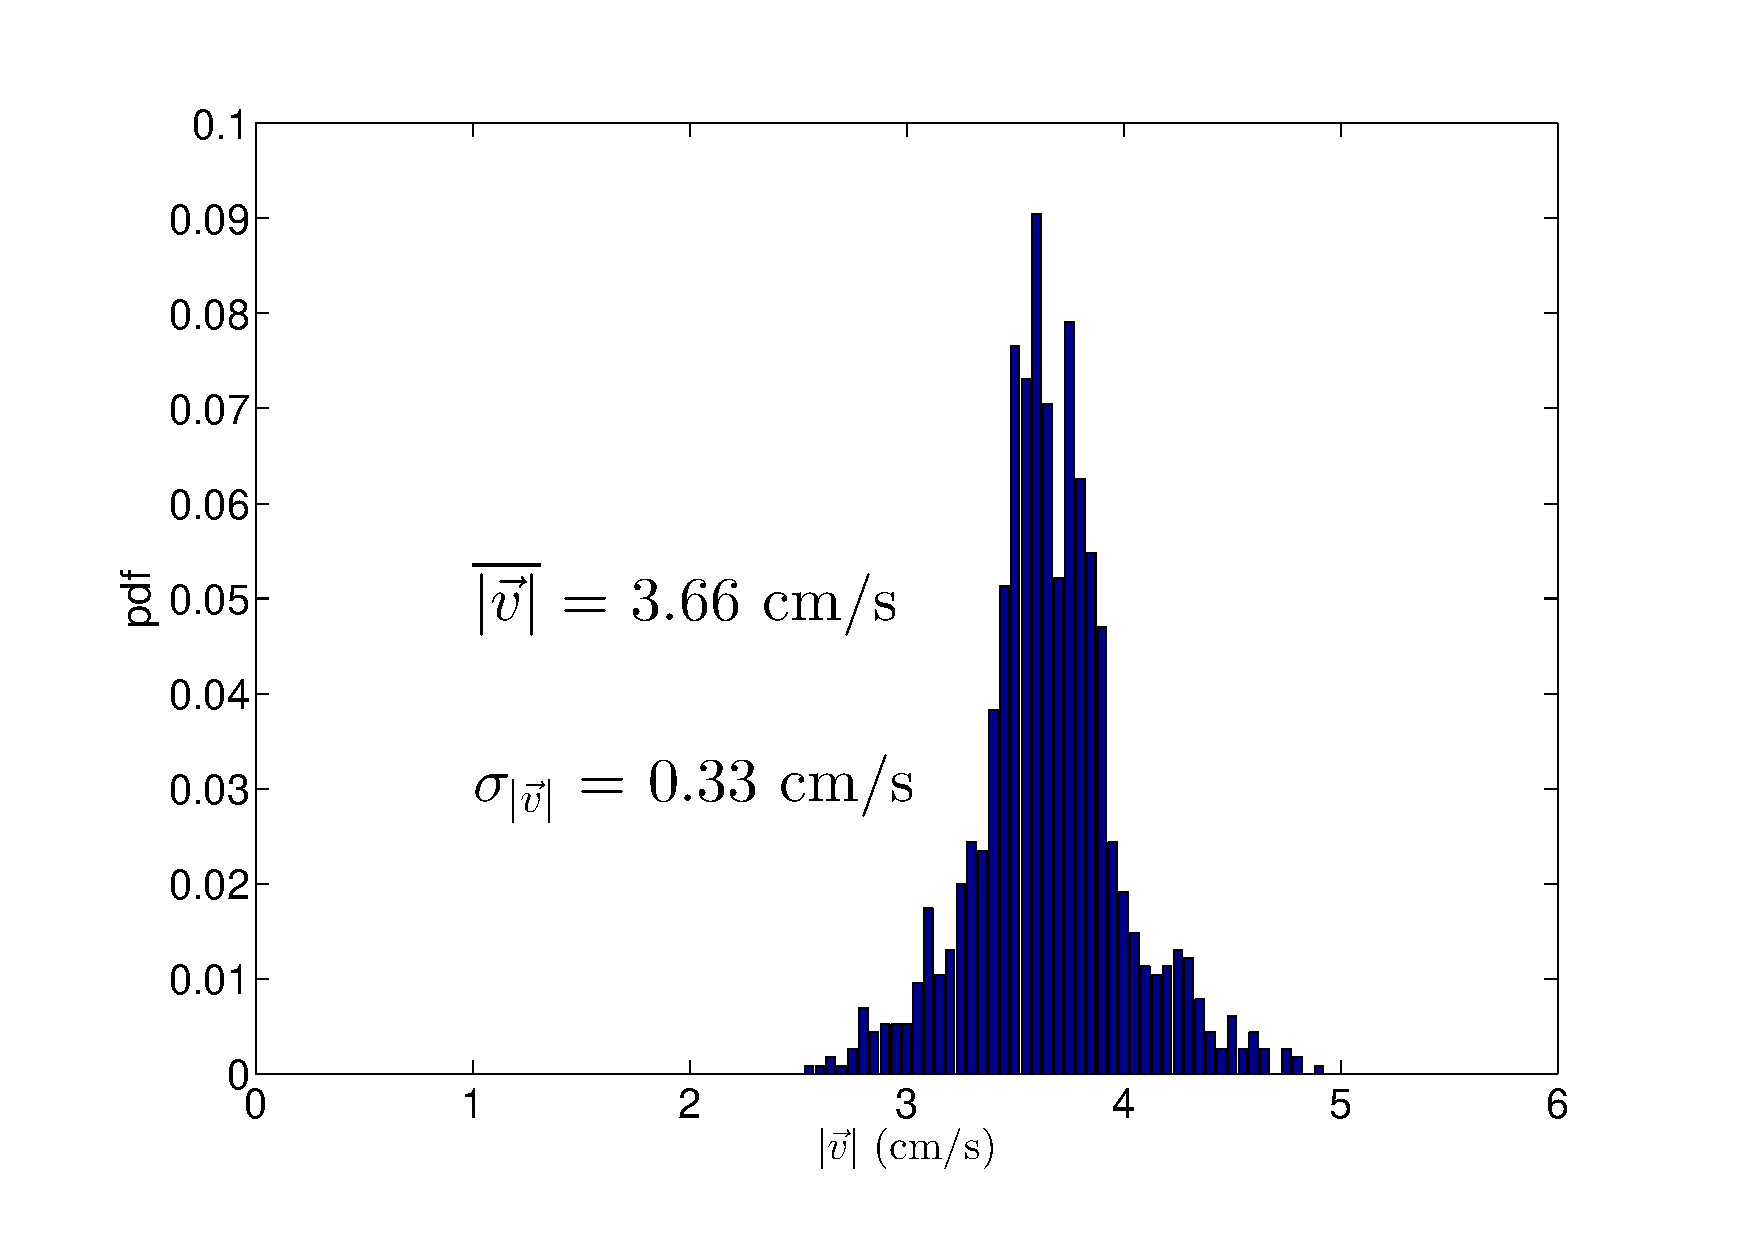
\includegraphics[scale=0.28]{cb_1_3mm_250mm_v_pdf.pdf}
       \caption{N = 1}
       \label{fig:vpdf_1_25}
	\end{subfigure}
	\hfill
	\begin{subfigure}[h!]{0.5\textwidth}
    \centering
       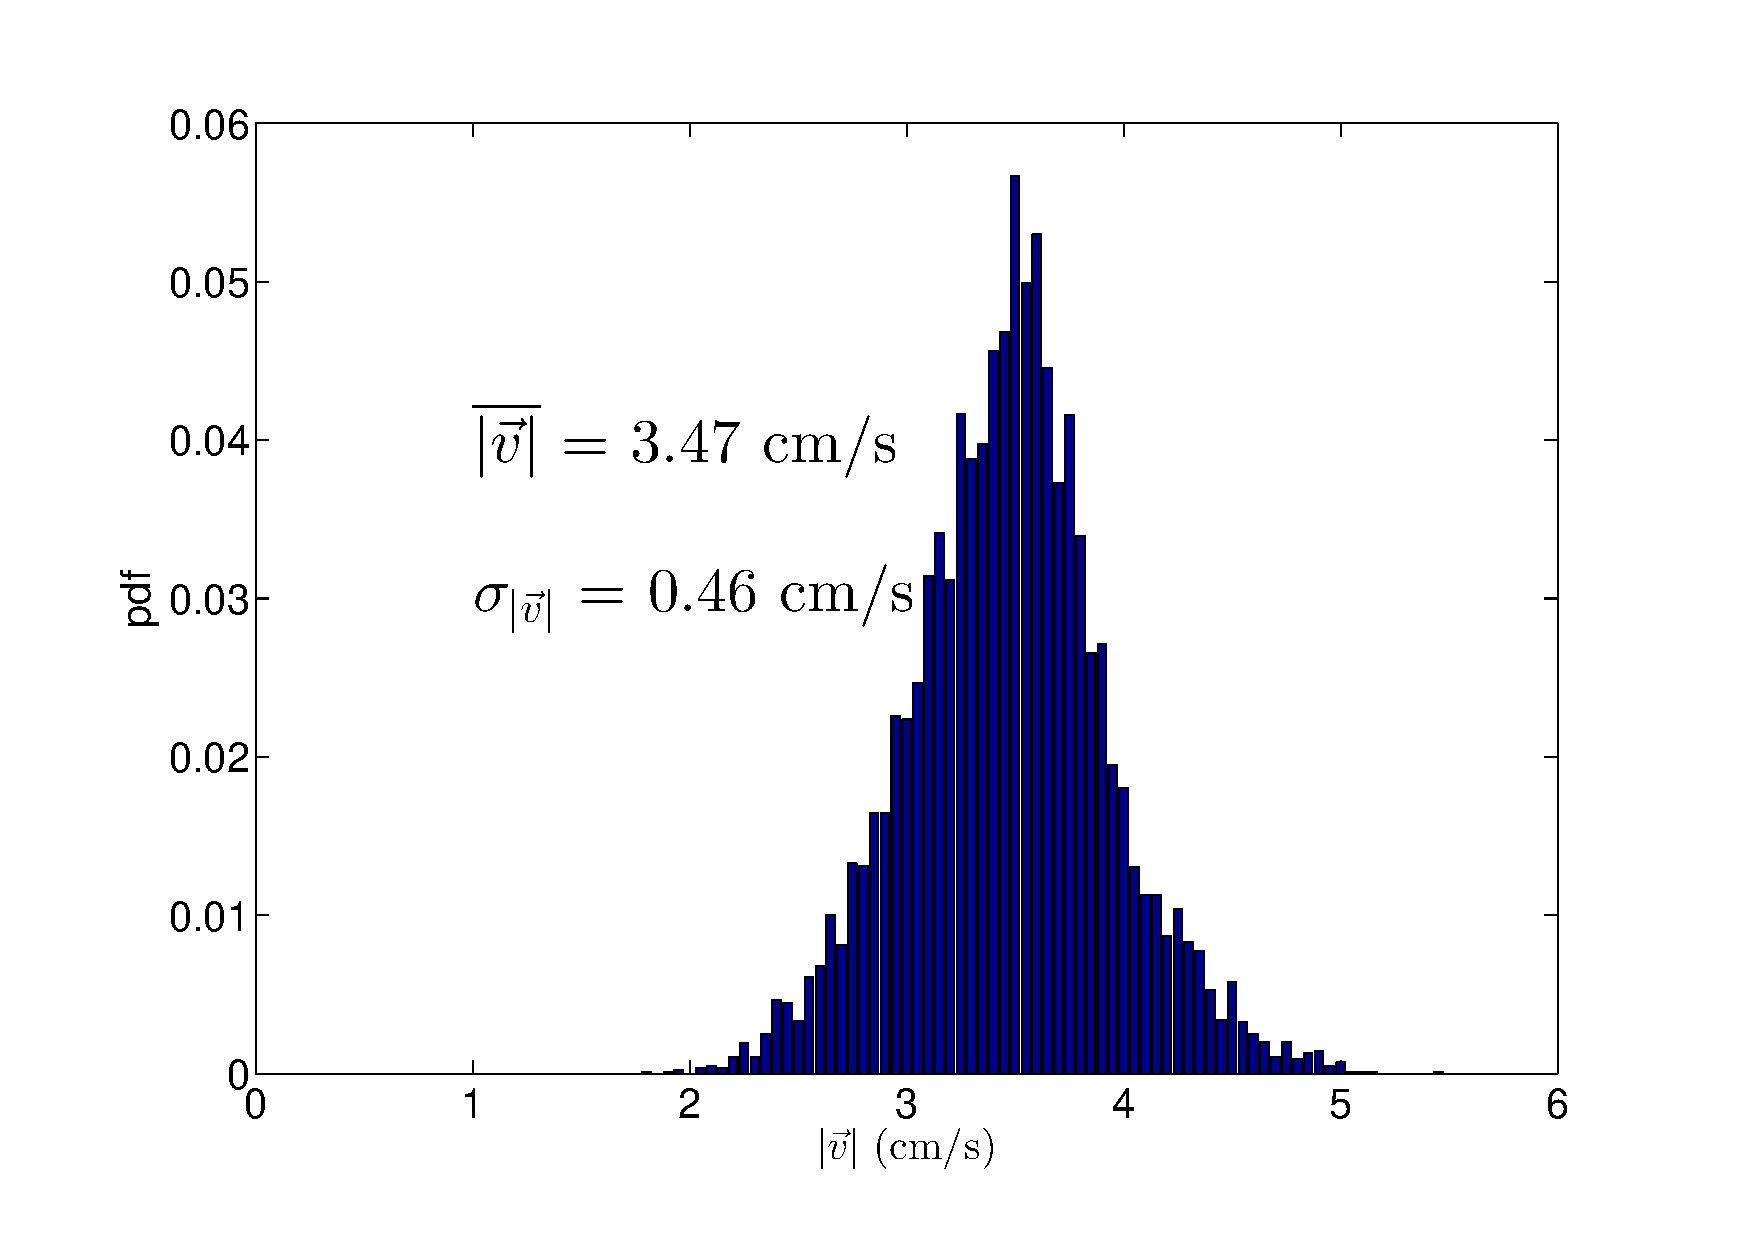
\includegraphics[scale=0.28]{cb_2_3mm_250mm_v_pdf.pdf}
       \caption{N = 2}
       \label{fig:vpdf_2_25cm}
	\end{subfigure}
	\begin{subfigure}[h!]{0.5\textwidth}
    \centering
       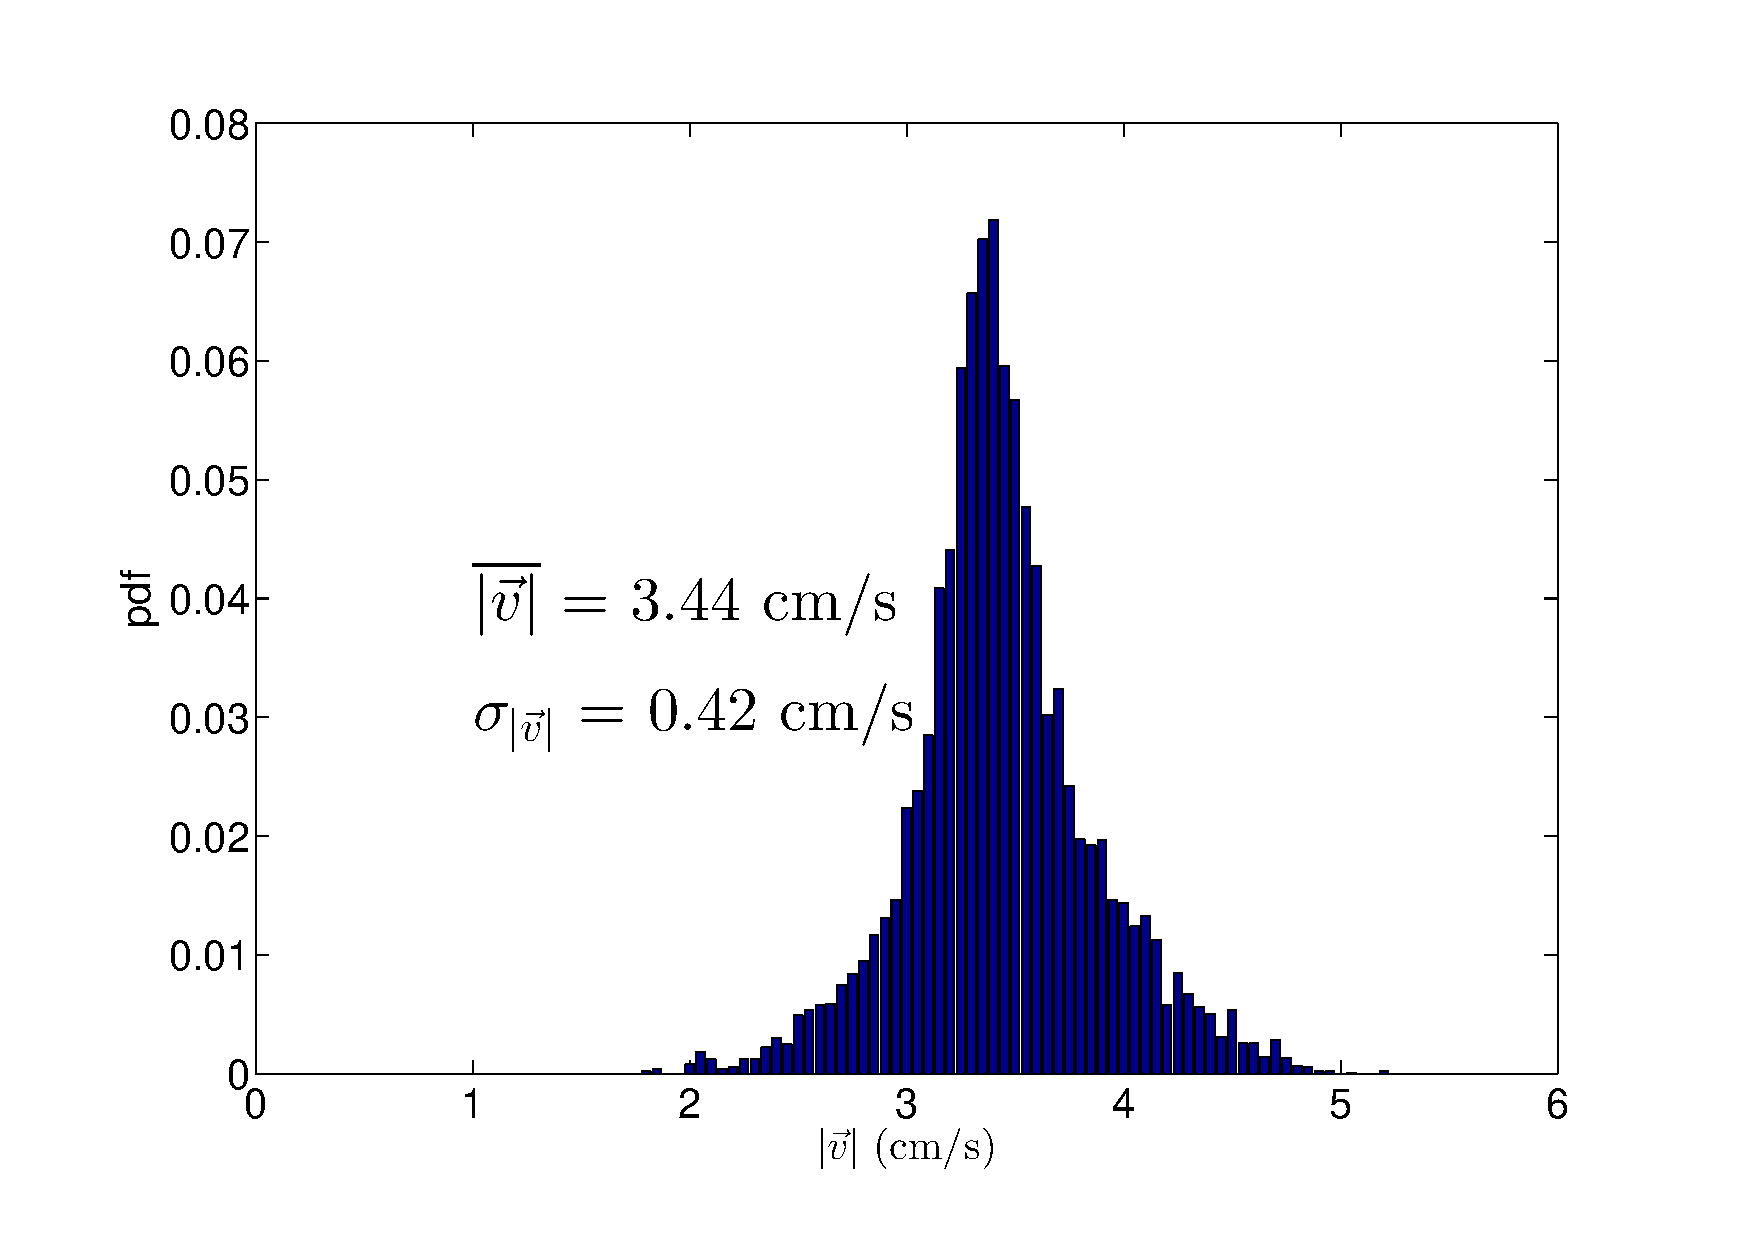
\includegraphics[scale=0.28]{cb_4_3mm_250mm_v_pdf.pdf}
       \caption{N = 4}
       \label{fig:vpdf_4_25cm}
	\end{subfigure}
	\hfill
	\begin{subfigure}[h!]{0.5\textwidth}
    \centering
       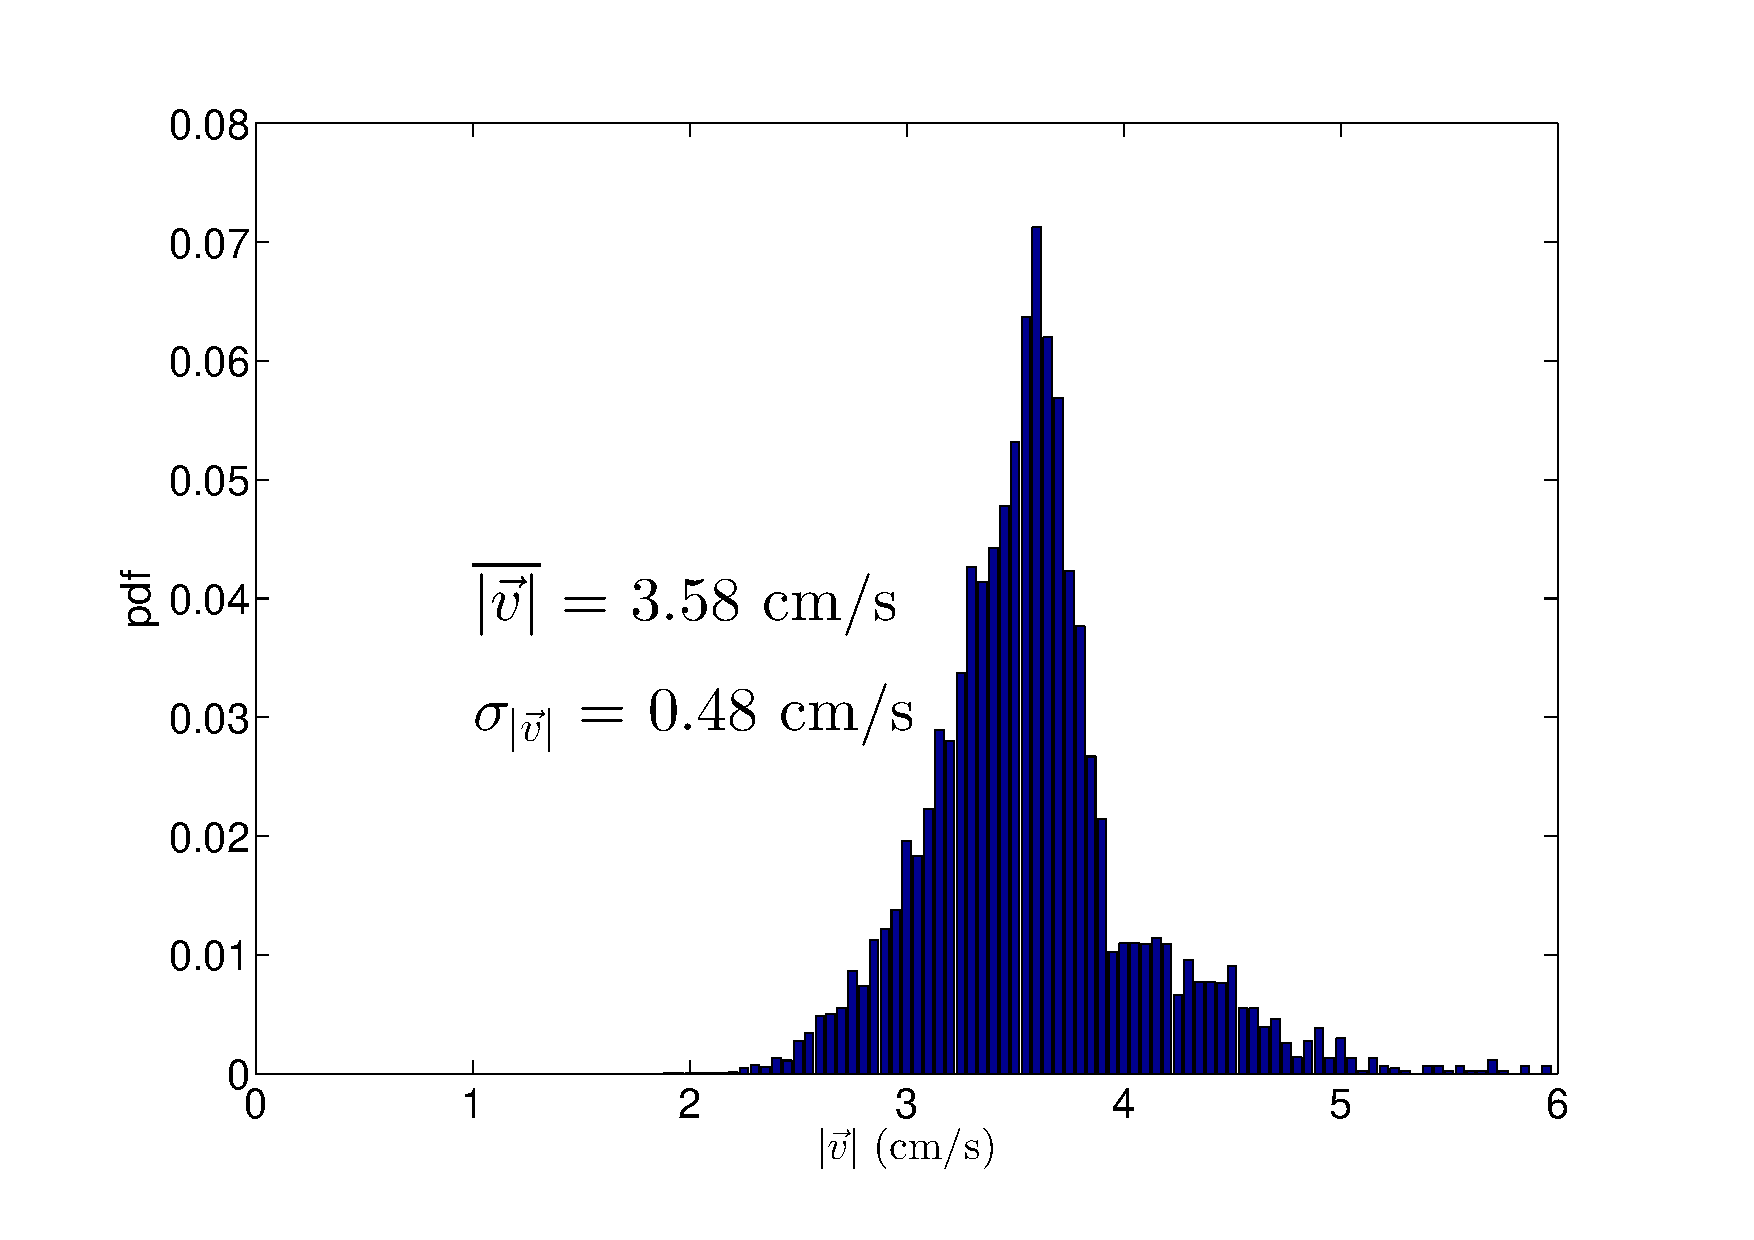
\includegraphics[scale=0.28]{cb_8_3mm_250mm_v_pdf.pdf}
       \caption{N = 8}
       \label{fig:vpdf_8_25cm}
	\end{subfigure}
	\begin{subfigure}[h!]{\textwidth}
    \centering
       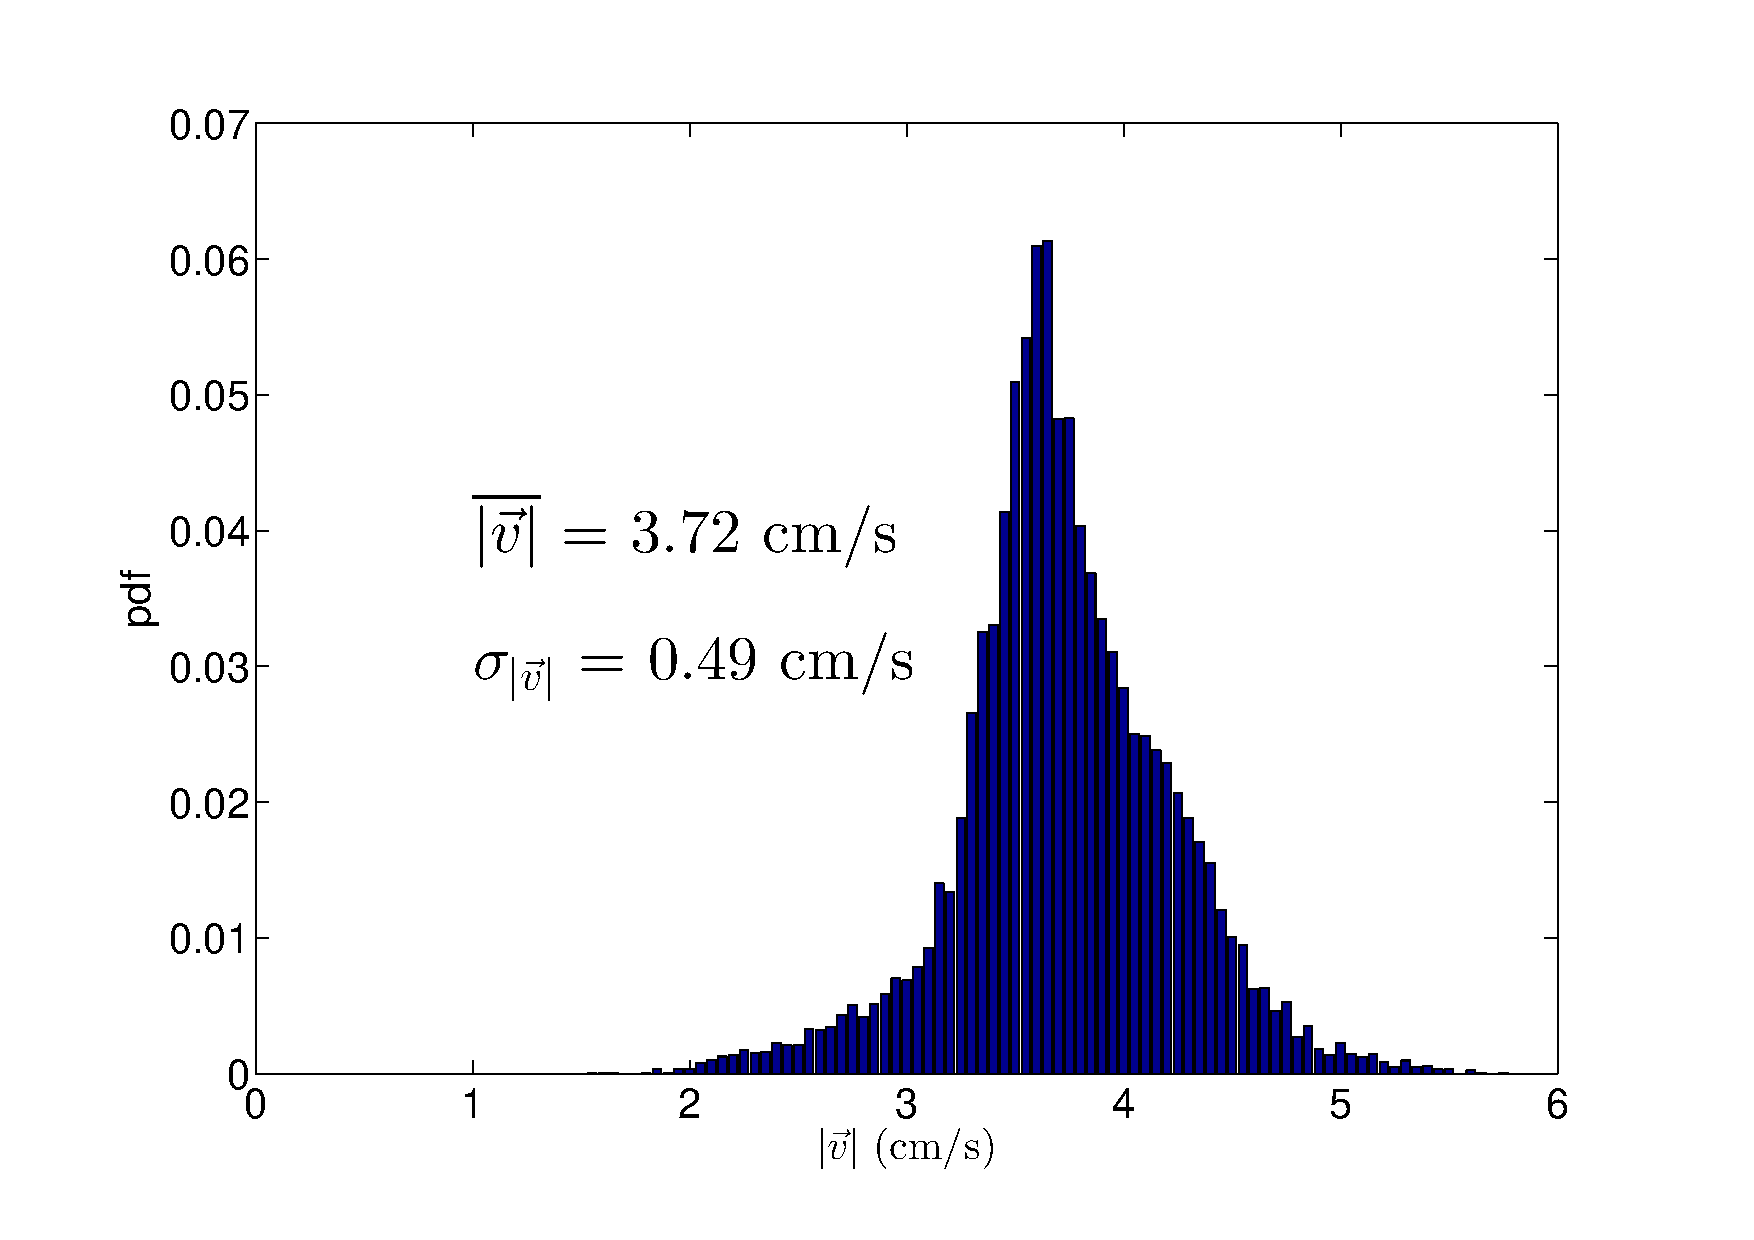
\includegraphics[scale=0.28]{cb_16_3mm_250mm_v_pdf.pdf}
       \caption{N = 16}
       \label{fig:vpdf_16_25cm}
	\end{subfigure}
	\caption{Average of speed distributions of 3 mm diameter c-boats in a 250 mm petri dish. The distribution does not change considerably because the system has not yet reached a critical packing density at which each of the c-boats feel the presence of the other c-boats.}
	\label{fig:vpdfall25cm}
\end{figure}

\subsection{Periodic Motion of the c-boats}
Another interesting phenomenon observed in the c-boat experiments is the periodic motion of the c-boat. Figure~\ref{fig:vsAll} shows the c-boat speed time traces at different intervals and the corresponding Power spectra. At the beginning of the experiment there is a strong peak at $\approx$ 1 Hz in the Power spectrum. The peak completely disappears at long times. What we cannot conclude is that, as time progresses whether the peak shifts to smaller frequencies or remains at 1 Hz while its amplitude decreases. In this section, we present a possible hypothesis to explain the source of the periodic motion. 
\begin{figure}[h!]
	\begin{subfigure}[h!]{0.5\textwidth}
    \centering
       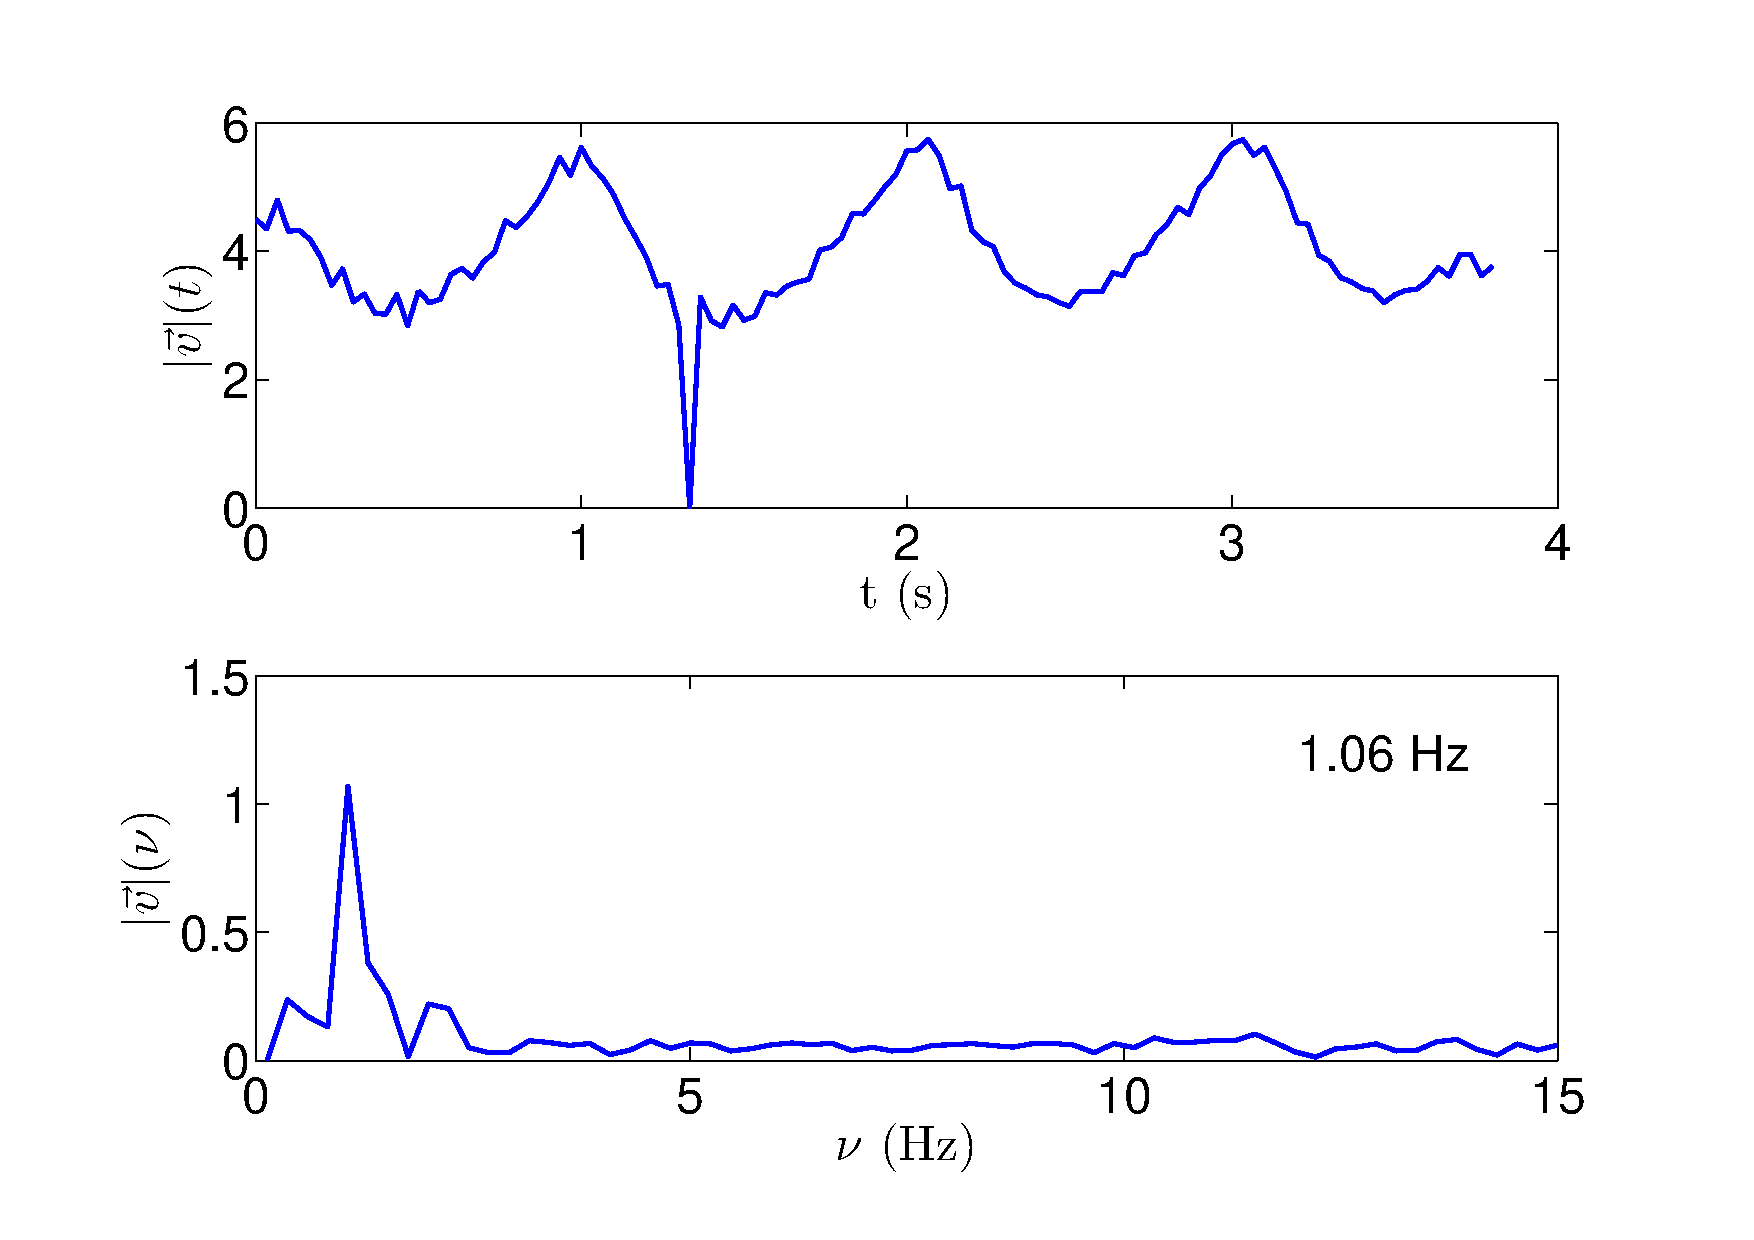
\includegraphics[scale=0.3]{voft_ps_0min.pdf}
       \caption{At 0 min}
       \label{fig:vs0min}
	\end{subfigure}
	\hfill
	\begin{subfigure}[h!]{0.5\textwidth}
    \centering
       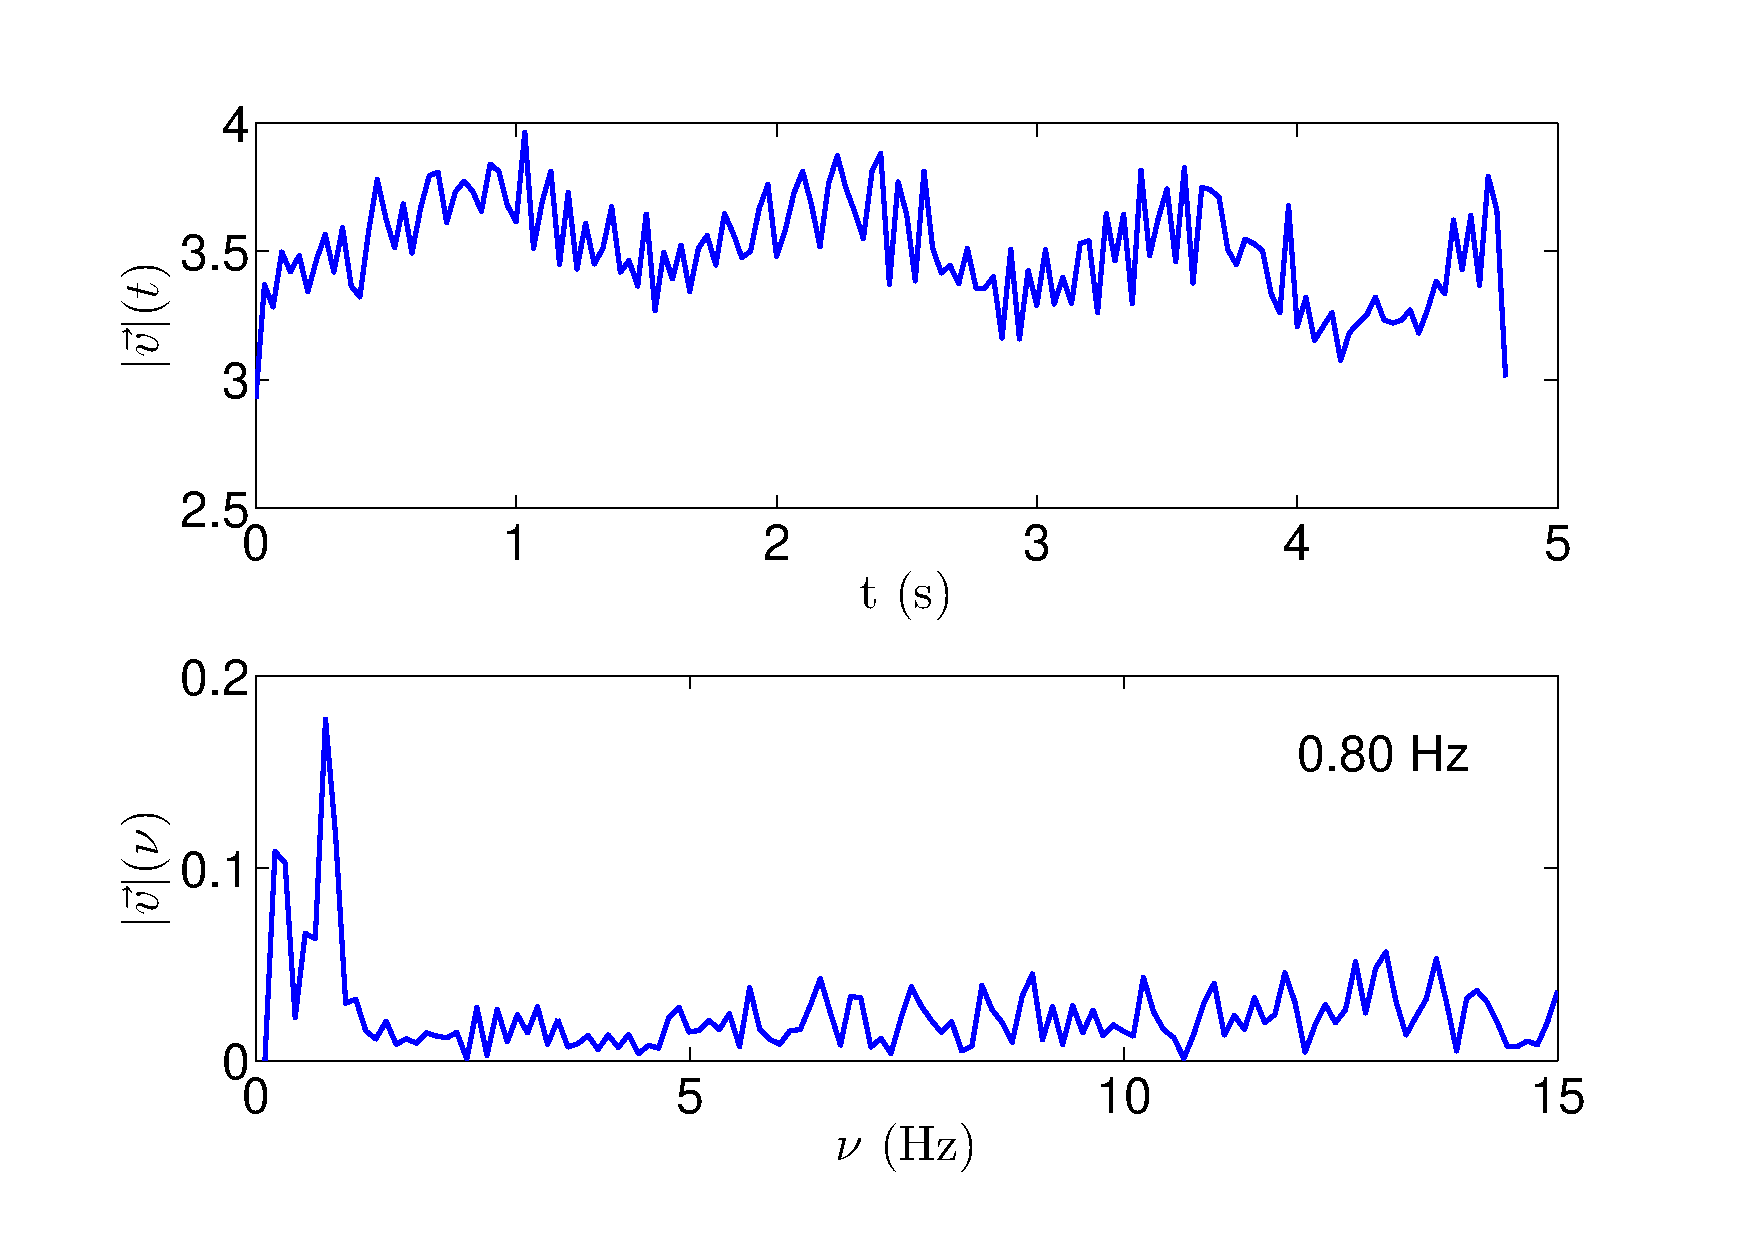
\includegraphics[scale=0.3]{voft_ps_5min.pdf}
       \caption{At 5 min}
       \label{fig:vs5min}
	\end{subfigure}
	\newline
	\begin{subfigure}[h!]{0.5\textwidth}
    \centering
       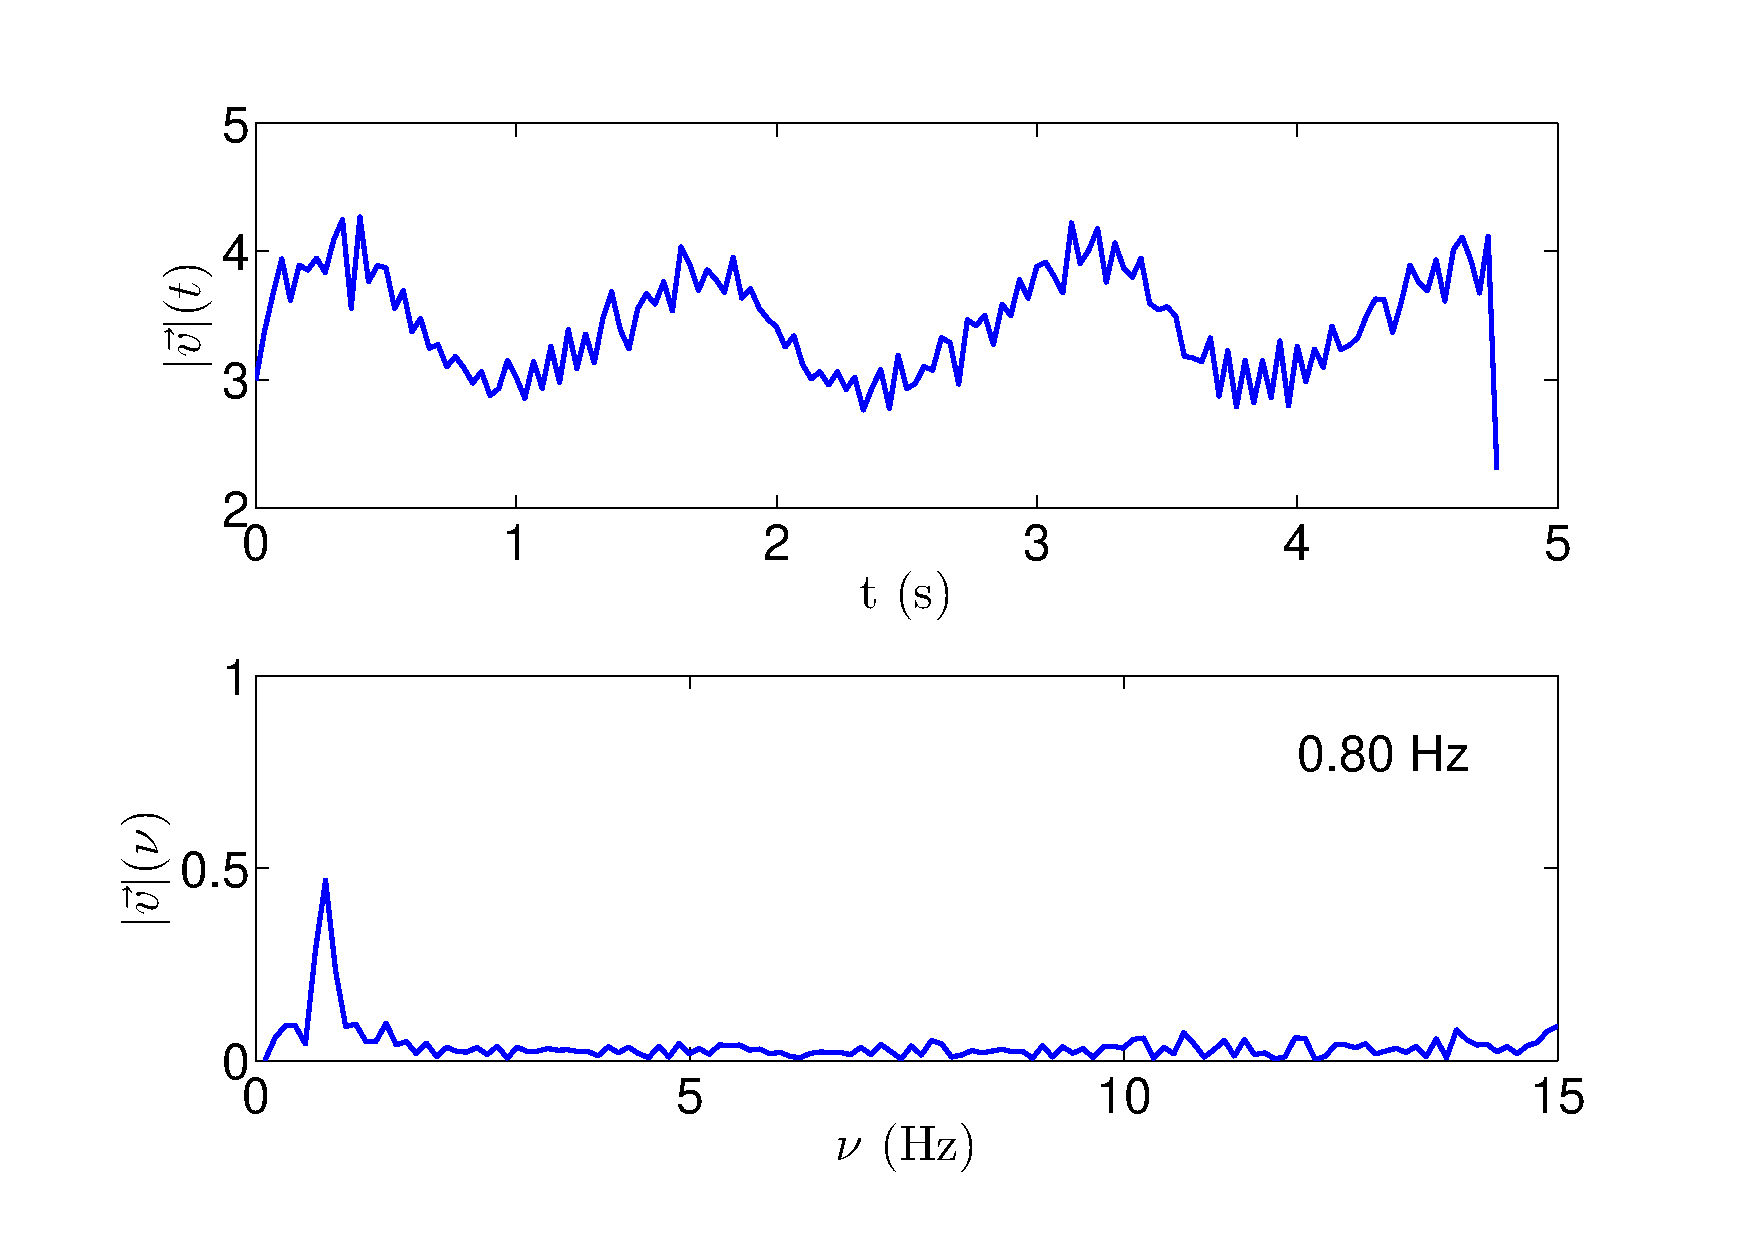
\includegraphics[scale=0.3]{voft_ps_10min.pdf}
       \caption{At 10 min}
       \label{fig:vs10min}
	\end{subfigure}
	\hfill
	\begin{subfigure}[h!]{0.5\textwidth}
    \centering
       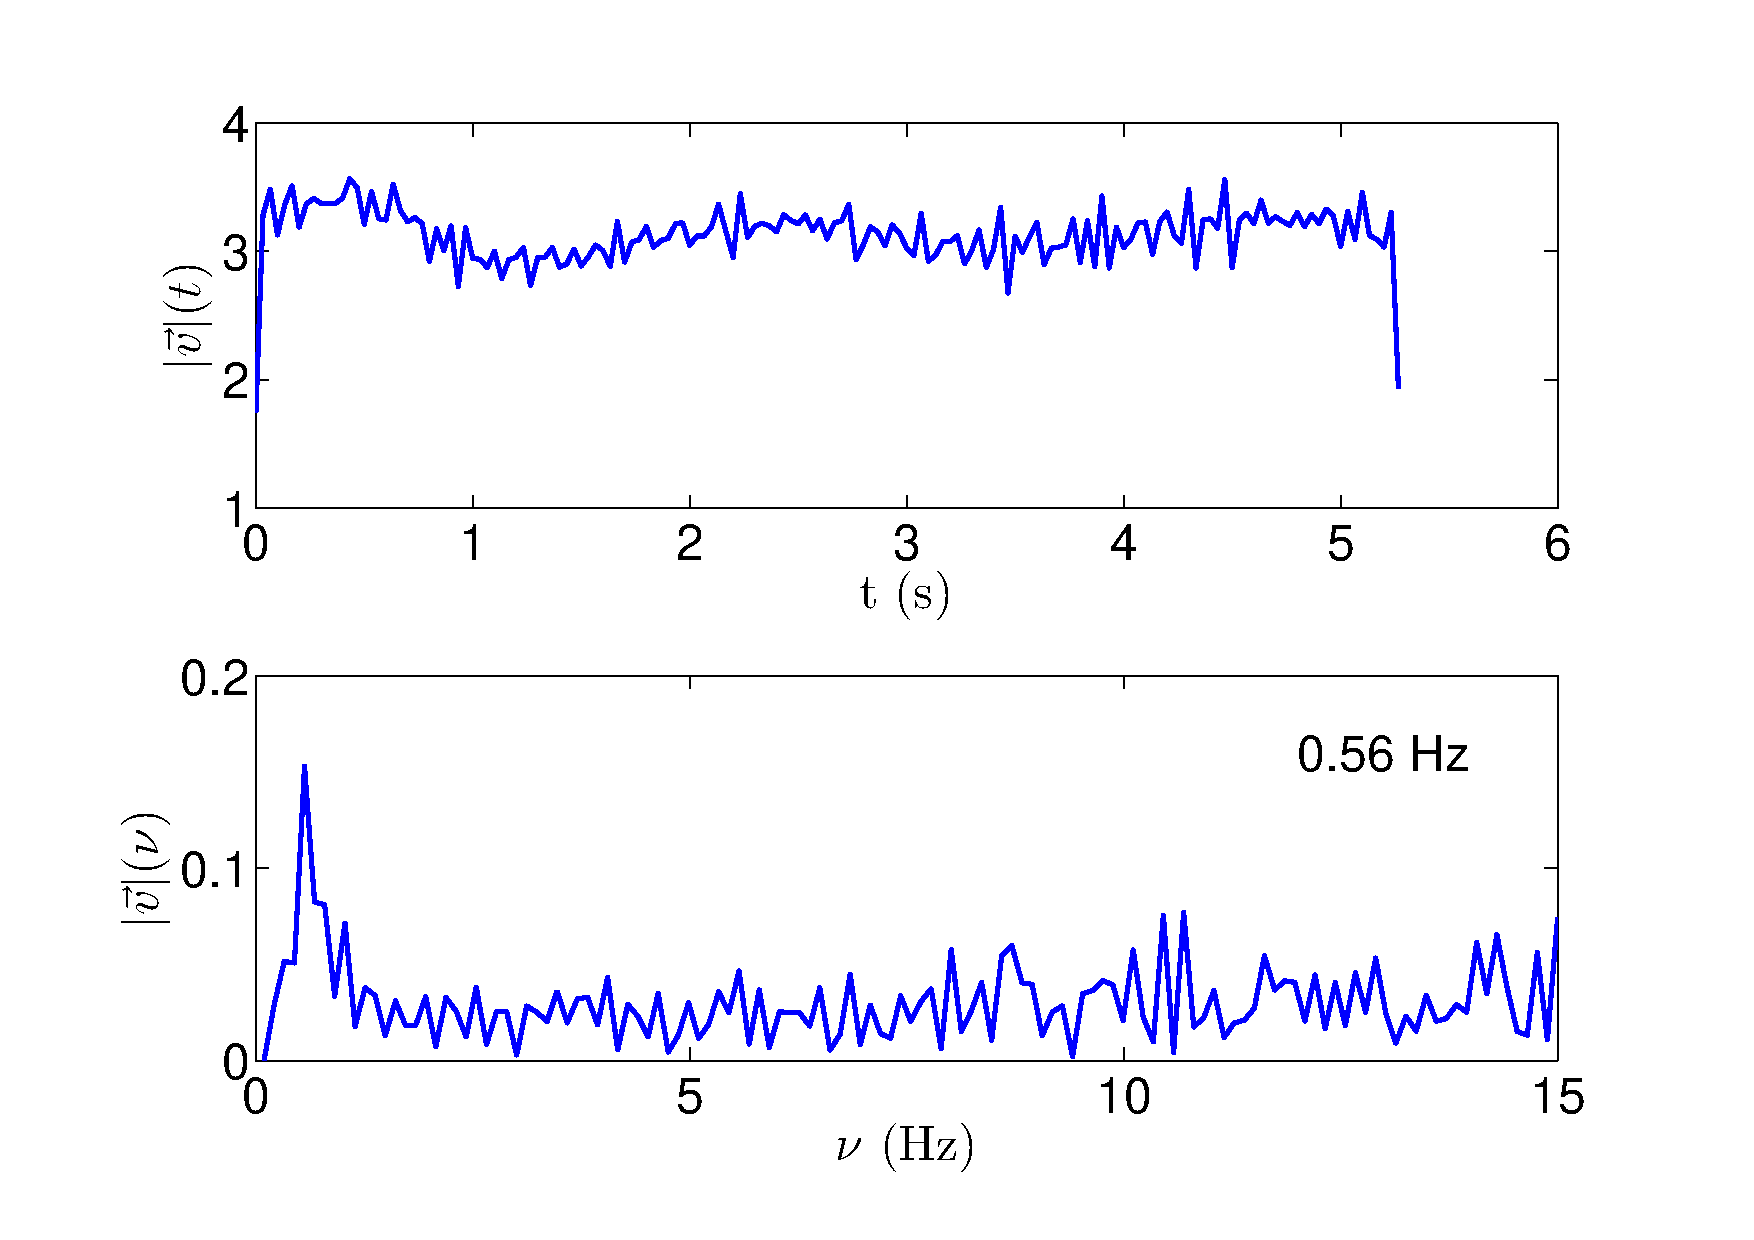
\includegraphics[scale=0.3]{voft_ps_20min.pdf}
       \caption{At 20 min}
       \label{fig:vs20min}
	\end{subfigure}
	\newline
	\begin{subfigure}[h!]{\textwidth}
    \centering
       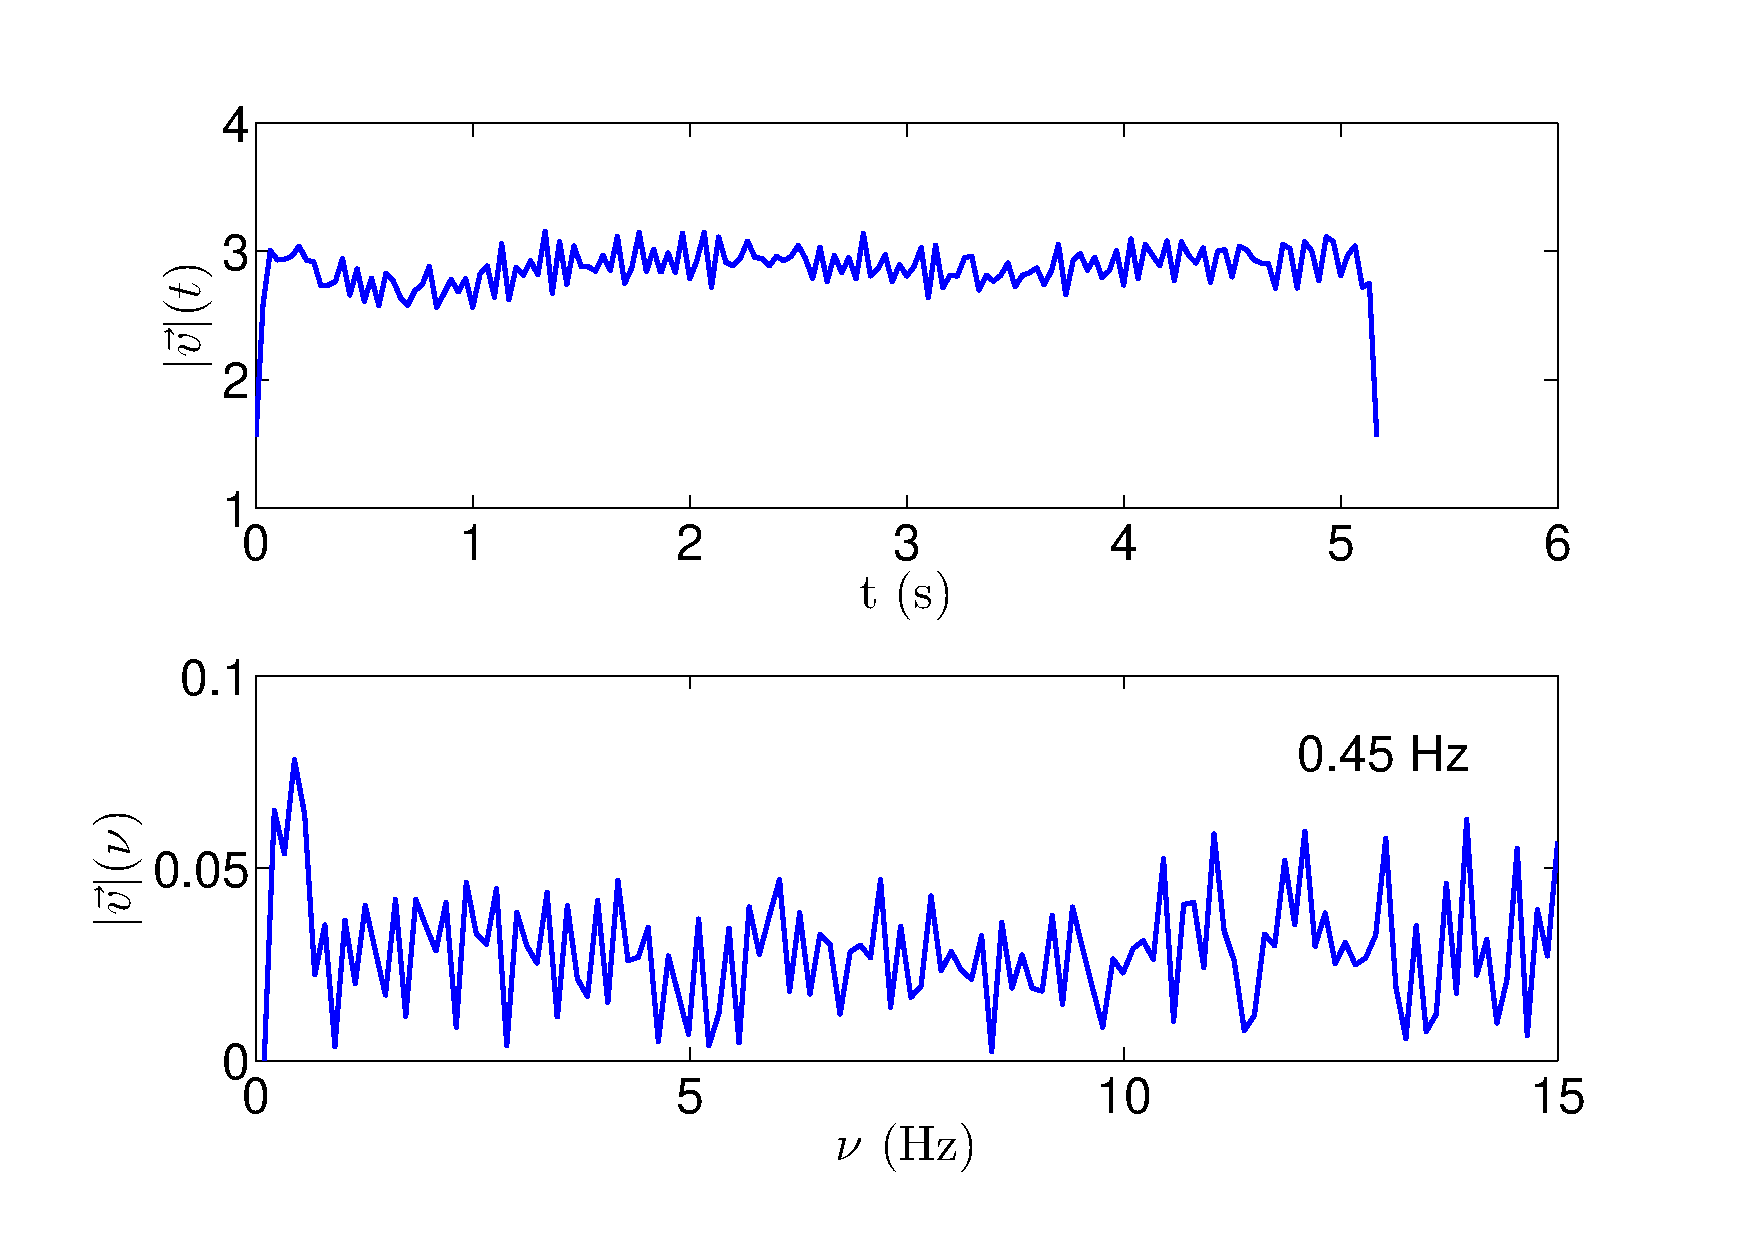
\includegraphics[scale=0.3]{voft_ps_30min.pdf}
       \caption{After 30 min}
       \label{fig:vs30min}
	\end{subfigure}
	\caption{Speed and Power spectrum of the speed at different times.}
	\label{fig:vsAll}
\end{figure}
One can also observe this effect, although indirectly, in the speed distribution of the c-boat at different intervals. Figure~\ref{fig:vpdf0and65} shows the speed distribution at the beginning and at long times of the c-boat. The speed distribution at the beginning shows a spread in the distribution due to to the periodic motion while at long times the distribution is gaussian. 

\begin{figure}[h!]
	\begin{subfigure}[h!]{0.5\textwidth}
    \centering
       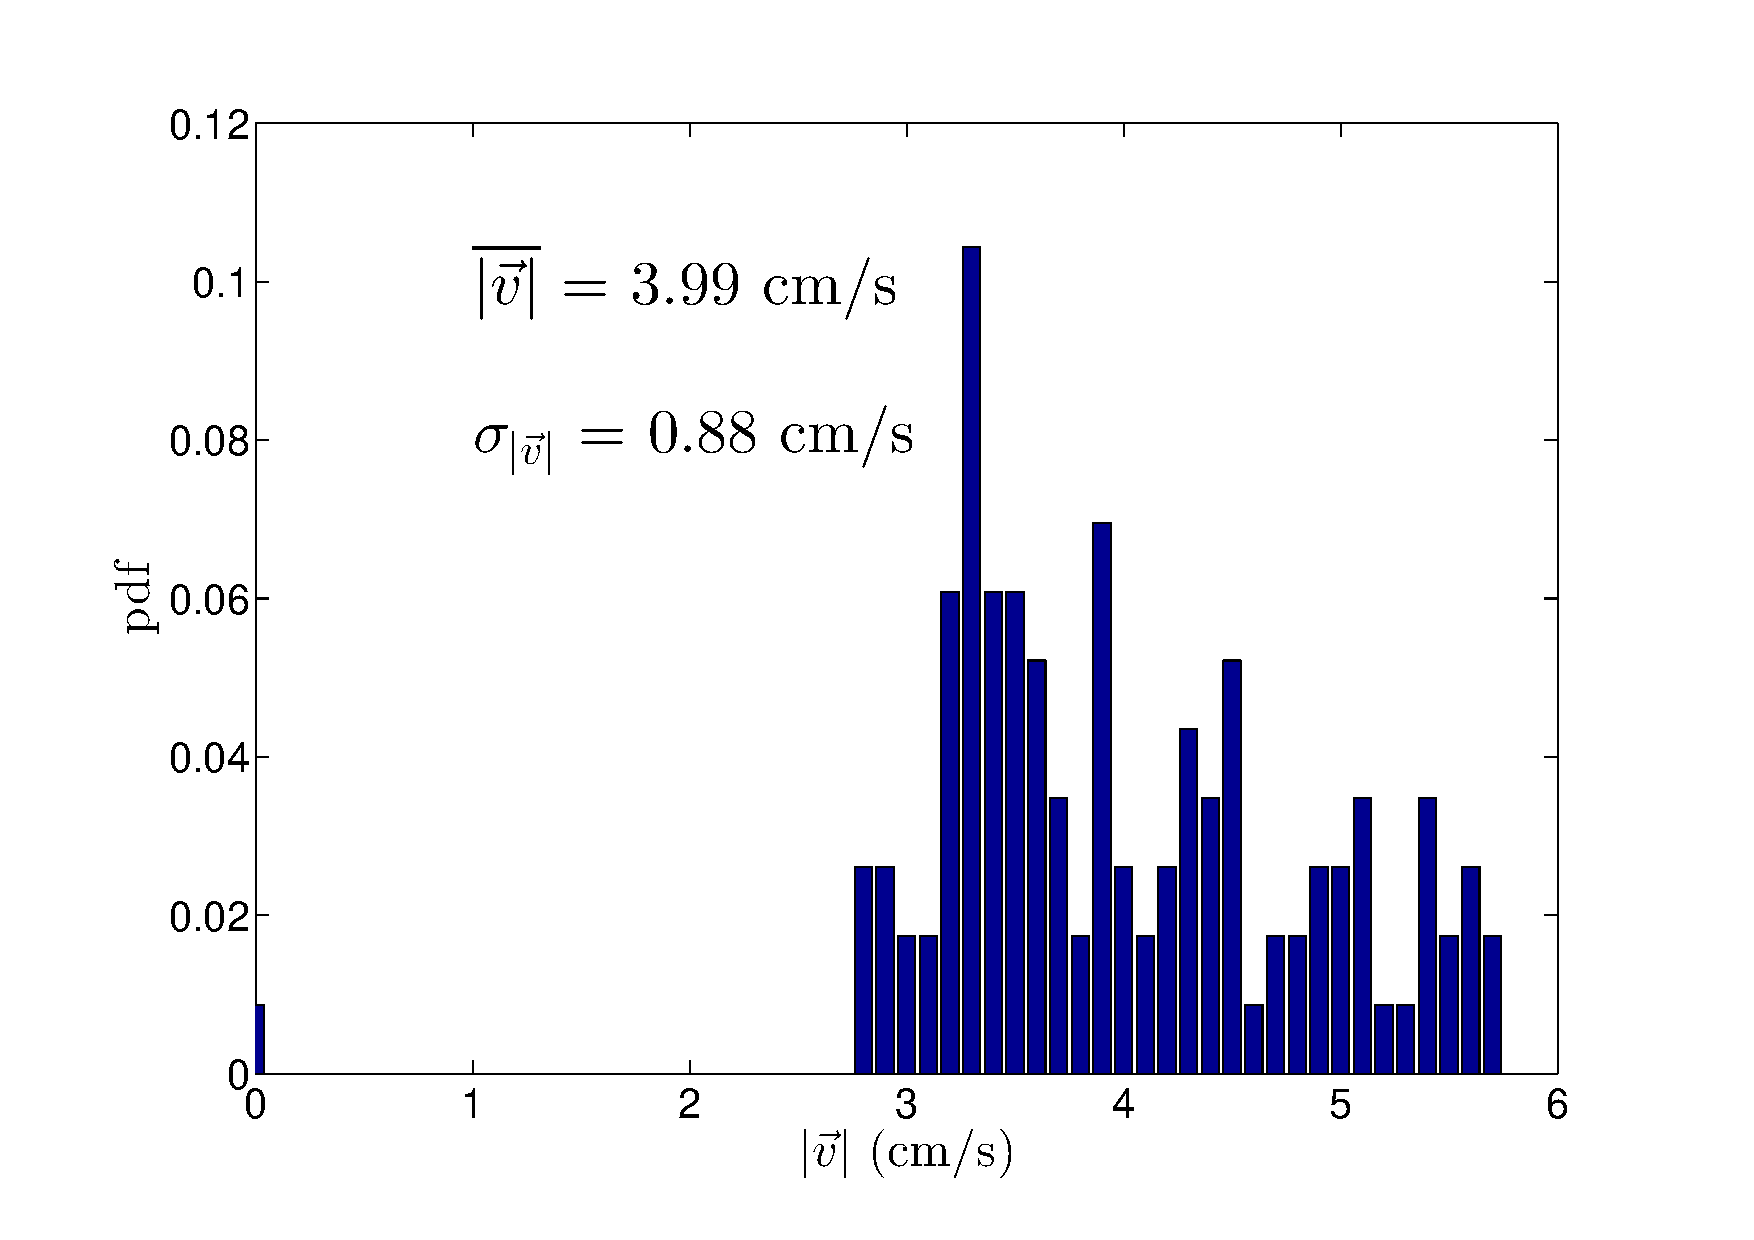
\includegraphics[scale=0.3]{cb_1_v_pdf_0min.pdf}
       \caption{At 0 min}
       \label{fig:vpdf0min}
	\end{subfigure}
	\hfill
	\begin{subfigure}[h!]{0.5\textwidth}
    \centering
       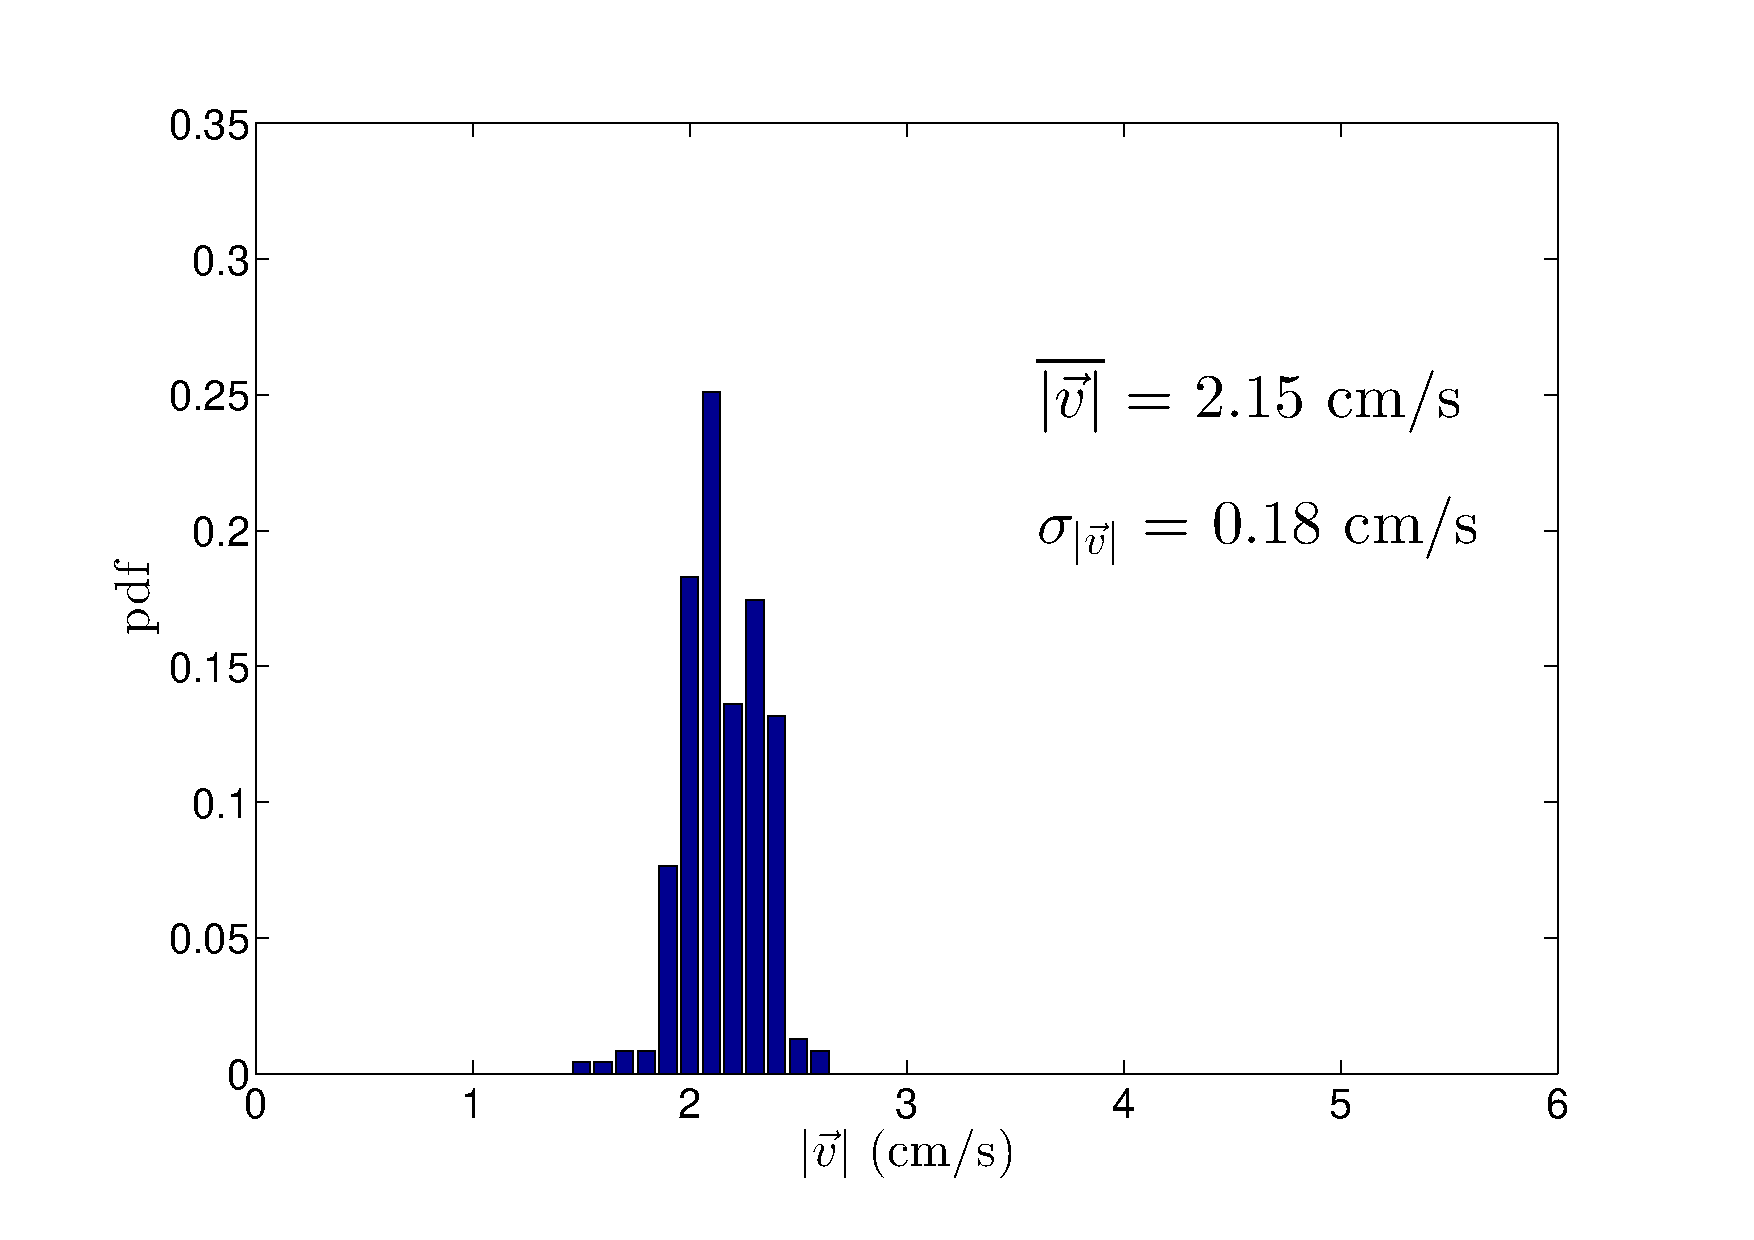
\includegraphics[scale=0.3]{cb_1_v_pdf_65min.pdf}
       \caption{At 65 min}
       \label{fig:vpdf65min}
	\end{subfigure}
	\caption{Speed distributions of a c-boat at small times (0 min) and at later times (65 min). The spread in the speed distribution at small times is another manifestation of the periodic motion of the c-boat.}
	\label{fig:vpdf0and65}
\end{figure}

From basic kinematics in 1-D, we have $v(t) = v_{0}+ at$, where $v_{0}$ is the initial velocity and $a$ is the acceleration. When two forces $F_{\eta}$ and $F_{\gamma}$ are acting the particle then, 
\begin{equation}
v = v_{0} + \left(\frac{F_{\eta} + F_{\gamma}}{m}\right) t
\end{equation}

where, $F_{\eta} = -k_{\eta}v$ is the drag force and $F_{\gamma}$ is the Marangoni force and $m$ is the mass of the particle.
\begin{align}
v &= v_{0} + \left(\frac{-k_{\eta}v + F_{\gamma}}{m}\right)t \nonumber \\
v + \frac{k_{\eta}v}{m}t &= v_{0} + \frac{F_{\gamma}}{m}t \nonumber \\
v &= \frac{v_{0}+\frac{F_{\gamma}}{m}t}{1+\frac{k_{\eta}}{m}t} \label{eq:vgen}
\end{align}

Equation~\ref{eq:vgen} is a general form of velocity/speed for the motion of any particle. Since the c-boat experiences the drag force, $F_{\eta}$ at all times, the observed periodic change in the velocity/speed of the c-boat must be due to the nature of the interfacial forces, $F_{\gamma}$. The c-boat moves to a location of lower camphor concentration. In order to move, the c-boat must overcome the drag forces. Therefore, until enough interfacial tension gradient is set up to overcome the drag force the c-boat does not accelerate. Once the drag forces are overcome, the c-boat accelerates (due to $F_{\gamma}$) and then decelerates (due to $F_{\eta}$). This process repeats itself as long as there is camphor in the c-boat. This hypothesis assumes that the force, $F_{\gamma}$ acts only a short duration of time, $\tau$ and is impulsive in nature. Therefore, we can re-write equation~\ref{eq:vgen}
\begin{equation}\label{eq:vcboat}
v = \frac{v_{0}+\frac{F_{\gamma}}{m}\tau}{1+\frac{k_{\eta}}{m}t}
\end{equation}

The observed time period of the oscillation in the speed of the particle is the time taken to set up enough concentration gradient to overcome the drag force. To experimentally validate this hypothesis, we propose to change $F_{\gamma}$ which can be done by 1. lowering the surface tension of water using Sodium Dodecyl Sufate (SDS) which results in lesser surface gradients around the c-boat, 2. changing the temperature of the room to decrease or increase sublimation rate. 

\end{document}
